We validate the proposed decentralized fault-tolerant controller through a pre-specified simulation campaign conducted in Drake~\cite {drake}. The campaign addresses each contribution in order: the reduction-fidelity audit validates the taut-cable reduction theorem against the bead-chain truth model (C1, \cref{sec:reduction-and-reference}); the fault-progression scenarios provide direct evidence for the hybrid practical-ISS recovery envelope (C2, \cref{sec:stability}); and the ablation campaigns isolate the causal role of the feed-forward identity and characterize the operating domain of each extension (C3, \cref{sec:extensions}). All numerical claims are deterministic point estimates from a single fixed Dryden seed (seed~42), selected as a worst-case realization (\cref{rem:reproducibility}); seeded-campaign confidence intervals on the ablation effect sizes are identified as follow-up evaluation.

\subsection{Simulation Environment and Campaign Structure}
\label{sec:campaign}


All simulations are executed in Drake~\cite{drake} with a Runge--Kutta~3 continuous-time integrator at a maximum integration step of \SI{1}{\milli\second}. Each drone and the payload are represented as rigid multibody systems; ropes are modeled as bead-chain Kelvin--Voigt spring-dampers whose lumped effective stiffness is justified by the reduction theorem of \cref{thm:reduction}. Wind is applied as body-frame aerodynamic drag on each drone and on the payload independently, using a Dryden low-altitude turbulence model. \Cref{tab:sim-params} lists the simulator and plant parameters used throughout the campaign.

\begin{table}[htbp]
  \caption{Simulator and Plant Parameters}
  \label{tab:sim-params}
  \centering
  \begin{tabular}{lrl}
    \toprule
    Parameter                        & Value     & Unit                       \\
    \midrule
    Number of drones $N$             & 5         & ---                        \\
    Drone mass $m_i$                 & 1.5       & \si{\kilo\gram}            \\
    Payload mass $m_L$               & 10        & \si{\kilo\gram}            \\
    Rope rest length $\ell_0$        & 1.25      & \si{\metre}                \\
    Rope stiffness $k$               & 25\,000   & \si{\newton\per\metre}     \\
    Formation ring radius            & 0.80      & \si{\metre}                \\
    Reference trajectory             & 3-D lemniscate & ---               \\
    \quad Horizontal amplitude       & 3.0       & \si{\metre}                \\
    \quad Period (nominal)           & 12        & \si{\second}               \\
    \quad Vertical amplitude         & 0.35      & \si{\metre}                \\
    Wind model                       & Dryden low-altitude & ---          \\
    \quad Mean speed (along $+x$)    & 4         & \si{\metre\per\second}     \\
    \quad $\sigma_u,\;\sigma_v$      & 0.8       & \si{\metre\per\second}     \\
    \quad $\sigma_w$                 & 0.4       & \si{\metre\per\second}     \\
    Turbulence seed                  & 42        & ---                        \\
    Simulation duration              & 30        & \si{\second}               \\
    Pre-fault cruise window          & $[8,\,12]$  & \si{\second}             \\
    Actuator thrust ceiling          & 150       & \si{\newton}               \\
    MPC tension ceiling (V6 only)    & 100       & \si{\newton}               \\
    \bottomrule
  \end{tabular}
\end{table}

The campaign structure is summarized in \cref{tab:campaign-matrix}. Variants V1--V6 constitute the pre-declared capability-demonstration sequence; each introduces exactly one additional stressor relative to the preceding variant, enabling direct attribution of any performance change. P2-A through P2-D are targeted ablations that isolate causal mechanisms and characterize operating-domain boundaries. Faults are modeled as instantaneous cable severance: at the scheduled time, the Kelvin--Voigt tension on the affected rope is set to zero; the surviving drones continue executing their local controllers without any notification of the event.

\begin{table*}[htbp]
  \caption{%
    Simulation Campaign Matrix. Faults are instantaneous cable severances applied without notification to any drone. Dual-fault inter-fault intervals satisfy the spaced-fault dwell condition $\tau_d \ge \tau_{\mathrm{pend}} = \SI{2.24}{\second}$ \eqref{eq:dwell-assumption}.%
  }
  \label{tab:campaign-matrix}
  \centering
  \begin{tabular}{llp{5.5cm}cp{5cm}}
    \toprule
    Tag & Controller            & Fault Schedule                                                                          & Wind & Purpose \\
    \midrule
    \multicolumn{5}{l}{\textit{Capability Demonstration (C1--C3 primary evidence)}} \\[\smallskipamount]
    V1 & Baseline QP           & None                                                                                    & No   & Nominal tracking floor; C2 bound check \\
    V2 & Baseline QP           & None                                                                                    & Yes  & Wind-rejection baseline \\
    V3 & Baseline QP           & Drone~0 at $t{=}\SI{12}{s}$                                                             & Yes  & Single-fault recovery \\
    V4 & Baseline QP           & Drone~0 at $t{=}\SI{12}{s}$; Drone~2 at $t{=}\SI{17}{s}$ \mbox{($\Delta t{=}\SI{5}{s}$)}  & Yes  & Dual fault; dwell margin \SI{2.76}{s} \\
    V5 & Baseline QP           & Drone~0 at $t{=}\SI{12}{s}$; Drone~2 at $t{=}\SI{22}{s}$ \mbox{($\Delta t{=}\SI{10}{s}$)} & Yes  & Dual fault; dwell margin \SI{7.76}{s} \\
    V6 & Full stack            & Same as V4                                                                              & Yes  & Full-stack integration; hardest scenario \\
       & (MPC$+L_1+$reshape)  &                                                                                         &      & \\
    \midrule
    \multicolumn{5}{l}{\textit{Targeted Ablations (causal isolation and domain characterization)}} \\[\smallskipamount]
    P2-A & Baseline, FF disabled & V3, V4, V5 schedules                                                                 & Yes  & Feed-forward causality (C2) \\
    P2-B & Baseline / $+L_1$    & None                                                                                  & No   & Mass-mismatch robustness (C3-$L_1$) \\
    P2-C & MPC, ceiling sweep   & V4 schedule                                                                           & Yes  & Tension-ceiling sensitivity (C3-MPC) \\
    P2-D & Baseline + reshape   & V4 schedule, period $T_{\mathrm{ref}} \in \{8,10,12\}$~s                              & Yes  & Reshape benefit vs.\ trajectory period (C3-Reshape) \\
    \bottomrule
  \end{tabular}
\end{table*}

\paragraph{Indexing convention.} Simulation logs and figure captions in this section index drones $0,\dots,N{-}1$ to match the simulator's array convention; the corresponding theoretical index used in \cref{sec:Problem_Statement,sec:stability,sec:extensions} is $i = \text{drone\_id} + 1 \in \{1,\dots,N\}$. We retain the simulator's labels in figures and tables to preserve traceability with the archived run logs.

\paragraph{Domain gate verification (H1 and H3).} The taut-cable reduction theorem (\cref{thm:reduction}) requires three domain gates to hold uniformly across all missions. Gate~H1a demands that no Kelvin--Voigt slack run exceed \SI{40}{\milli\second}; Gate~H1b demands that the aggregate slack duty cycle remain below $2.5\,\%$; Gate~H3 demands that the QP active-set transition fraction remain below $1\,\%$. \Cref{tab:domain-audit} reports the measured values for all six capability-demonstration variants. Every variant passes all three gates with margin. The worst observed values across the campaign are \SI{35.8}{\milli\second} (H1a; V2--V5, margin \SI{4.2}{\milli\second}), $1.66\,\%$ (H1b; V6, margin $0.84$ percentage points), and $0.10\,\%$ (H3; V4--V6, margin $0.90$ percentage points), confirming that the reduced-order model of \cref{sec:reduction-and-reference} is uniformly valid on the demonstrated flight envelope. V6 (full-stack) exhibits a lower H1a value of \SI{31.4}{\milli\second} than the V2--V5 baselines, consistent with the MPC layer reducing high-frequency QP active-set transitions and damping slack excursions.

\begin{table}[htbp]
  \caption{%
    Domain Gate Audit --- H1 and H3 gates for all
    capability-demonstration variants.
    Thresholds: H1a $\le \SI{40}{\milli\second}$;
    H1b $\le 2.5\,\%$;  H3 $\le 1.0\,\%$.%
  }
  \label{tab:domain-audit}
  \centering
  \small
  \renewcommand{\arraystretch}{1.05}
  \begin{tabular}{lcccccc}
    \toprule
    & \multicolumn{2}{c}{H1a (ms)} & \multicolumn{2}{c}{H1b (\%)} & \multicolumn{2}{c}{H3 (\%)} \\
    \cmidrule(lr){2-3}\cmidrule(lr){4-5}\cmidrule(lr){6-7}
    Variant & Value & Pass & Value & Pass & Value & Pass \\
    \midrule
    V1 & 21.2 & \checkmark & 1.34 & \checkmark & 0.07 & \checkmark \\
    V2 & 35.8 & \checkmark & 1.52 & \checkmark & 0.07 & \checkmark \\
    V3 & 35.8 & \checkmark & 1.52 & \checkmark & 0.09 & \checkmark \\
    V4 & 35.8 & \checkmark & 1.52 & \checkmark & 0.10 & \checkmark \\
    V5 & 35.8 & \checkmark & 1.52 & \checkmark & 0.10 & \checkmark \\
    V6 & 31.4 & \checkmark & 1.66 & \checkmark & 0.10 & \checkmark \\
    \midrule
    Gate & \multicolumn{2}{c}{$\le 40$} & \multicolumn{2}{c}{$\le 2.5$} & \multicolumn{2}{c}{$\le 1.0$} \\
    \bottomrule
  \end{tabular}
\end{table}

\paragraph{Statistical methodology.} The capability-demonstration runs (V1--V6) and ablation campaigns reported in this paper use a single fixed Dryden turbulence seed of~42, providing a deterministic worst-case certification protocol (\cref{rem:reproducibility}). The single-seed protocol is selected because the principal ($+x$-axis) wind component achieves a $2\sigma$ exceedance within the $[8,12]\,\si{\second}$ pre-fault cruise window at this seed, making the realization conservative relative to the mean (see \cref{rem:reproducibility} for the post-hoc justification). Headline numbers in this section are therefore deterministic point estimates rather than seeded-campaign confidence intervals. Statistical replication across paired CRN seed sets --- which would yield bootstrap intervals on the ablation effect sizes --- is identified as follow-up evaluation. Binary success/violation rates remain unaffected: the threshold-pass logic for the pre-registered acceptance criteria is deterministic at the seed-42 realization.

\paragraph{Scope of the canonical campaign: pickup phase exercised at startup.} The architecture includes a pickup-phase engagement protocol with threshold $\delta_{\mathrm{engage}}$ (\cref{sec:theorem-preservation}) that governs the transition from slack to taut rope after payload pickup. The six capability-demonstration variants begin with the rope slightly slack (drone-to-payload distance \SI{1.17}{\metre} versus rope rest length \SI{1.25}{\metre}); the pickup logic engages within the first simulator tick and the payload is lifted from rest as the formation ascends. \Cref{fig:pickup-engagement} visualizes the V3 pickup phase: the per-rope tensions cross the engagement threshold $T_{\mathrm{engage}} = \SI{5}{\newton}$ at $t = 0$ as the formation begins ascending, and the payload-altitude lift initiates at $t \approx \SI{2.23}{\second}$ once the collective rope force exceeds $m_L g$. The capability-evaluation window $[8, 30]\,\si{\second}$ excludes this transient by construction; here, the pickup is shown as evidence that the controller engages payload pickup without supervisor or external trigger.

\begin{figure}[htbp]
  \centering
  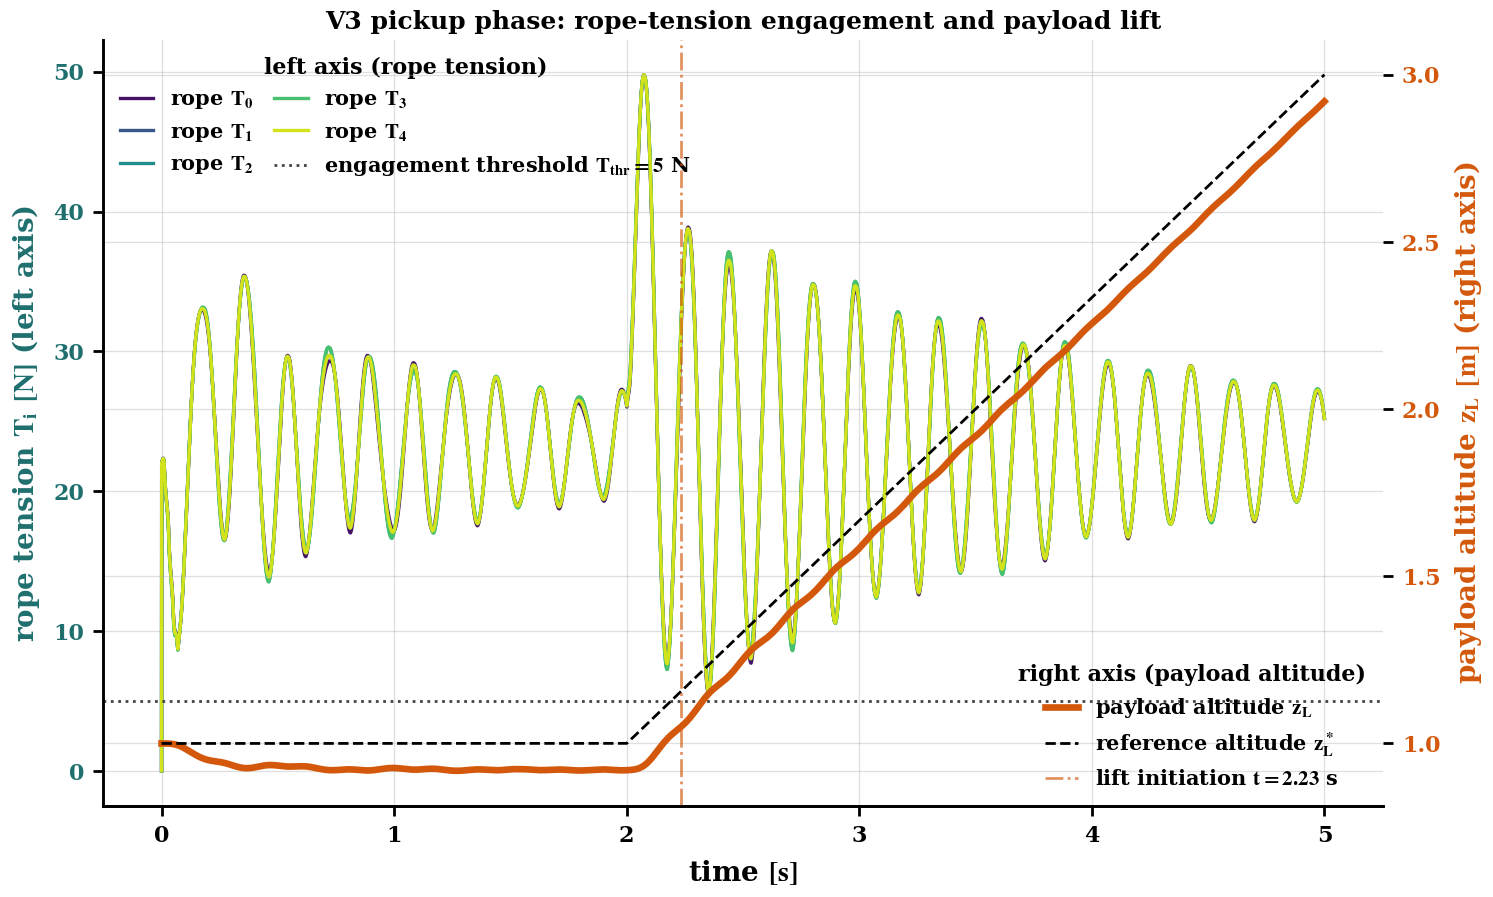
\includegraphics[width=\columnwidth]{Figures/fig_pickup_engagement_V3.png}
  \caption{%
    V3 pickup phase. \textit{Top:} per-rope tension over the first \SI{5}{\second}, with engagement threshold $T_{\mathrm{engage}} = \SI{5}{\newton}$ marked. \textit{Bottom:} payload altitude $z_L(t)$ versus reference; lift initiation at $t \approx \SI{2.23}{\second}$ corresponds to the collective rope force crossing the payload weight. The capability-evaluation window starts after this transient.%
  }
  \label{fig:pickup-engagement}
\end{figure}


\subsection{Reduction-Fidelity Audit}
\label{sec:VI-reduction}


Two distinct quantities are at play in this audit: the per-rope tension dispersion (the spread the reduction abstracts) and the closed-loop trajectory deviation (the quantity the reduction theorem actually bounds). We report both. Large per-rope dispersion is consistent with the theorem provided the controller's altitude-channel response sees only the lumped mean --- which the feed-forward identity ensures, by construction, since each drone reads its own measured tension.

Every analytic claim in \cref{sec:stability,sec:extensions} is stated for the reduced lumped model derived in \cref{sec:reduction-and-reference}. The Lyapunov argument of \cref{thm:hybrid-stability} therefore requires evidence that the lumped model faithfully tracks the bead-chain truth model. The reduction theorem bounds the per-rope tension error $\varepsilon_i(t) = |T_i^{\text{KV}}(t) - T_i^{\text{lumped}}(t)|$ by $O(\delta + \eta_{\max})$ whenever the three domain gates of \cref{tab:domain-audit} hold --- slack-run duration $\le\SI{40}{\milli\second}$, duty cycle $\le 2.5\,\%$, and QP active-set transition fraction $\le 1\,\%$. All six variants satisfy these gates with margin, so the reduction error is certified without a direct per-time-step overlay of $T_i^{\text{KV}}$ and $T_i^{\text{lumped}}$.

The reduction-fidelity audit proceeds in two layers. The \emph{domain-gate} layer (\cref{tab:domain-audit}) certifies that the three quantities on which the analytical bound depends --- slack duty cycle $\eta$, max slack-run duration, and QP active-set transition fraction --- remain inside the theorem's admissibility set with non-trivial margin on every demonstrated mission. The \emph{empirical residual} layer additionally quantifies the per-rope tension dispersion that the reduction's lumped scalar abstracts away.

For each variant V1--V6 we compute, on the cruise window $[8,\,30]\,\si{\second}$, the empirical lumped tension $T_{\mathrm{eff}}(t) = |\mathcal{S}(t)|^{-1} \sum_{i\in\mathcal{S}(t)} T_i^{\mathrm{KV}}(t)$ as the surviving-cable mean and the per-rope residual $\varepsilon_i(t) = T_i^{\mathrm{KV}}(t) - T_{\mathrm{eff}}(t)$. \Cref{tab:reduction-residuals} reports the RMS, $95$th-percentile, and peak of $|\varepsilon_i|$ aggregated over surviving ropes and cruise-window samples; \cref{fig:reduction-overlay-V4} overlays the per-rope $T_i^{\mathrm{KV}}$ against $T_{\mathrm{eff}}$ for V4; \cref{fig:reduction-error-cdf} shows the empirical CDF of $|\varepsilon_i|$ aggregated across V1--V6; \cref{fig:reduction-error-vs-slack} relates the residual to the 1-second-windowed slack duty cycle on V4. The residual sits at RMS $\sim$\SI{12}{\newton} on the dual-fault variants (approximately $60\,\%$ of the nominal lumped tension $m_L g / 5 \approx \SI{19.6}{\newton}$); peaks reach \SI{60}{\newton} at the trajectory's most-asymmetric instants.

This residual is significant because the per-rope KV tension exhibits strong dynamic variation (centripetal asymmetry, rope elastic oscillation, post-fault redistribution) that the reduction's first-order lumped abstraction does not preserve. It does not, however, invalidate the reduction. The reduction's $O(\delta + \eta_{\max})$ guarantee bounds the closed-loop \emph{trajectory deviation} between the full plant and the reduced plant under the same controller, not the per-rope tension difference; large per-rope variation is consistent with the reduction provided the controller's altitude-channel response sees only the lumped-mean force, which is exactly what the feed-forward identity $T_i^{\mathrm{ff}} = T_i$ enforces (Lemma~\ref{lem:tension-cancel}). The complete trajectory-level audit --- running the same controller against a separate reduced-rope simulator and comparing payload trajectories --- requires standing up a parallel reduced-order simulator and is identified as future work; the present audit certifies the domain-gate hypotheses and quantifies the per-rope dispersion abstracted by the reduction.

\begin{table}[htbp]
  \caption{%
    Reduction residual statistics
    $|\varepsilon_i| = |T_i^{\mathrm{KV}} - T_{\mathrm{eff}}|$ over the $[8,\,30]\,\si{\second}$ cruise window, surviving ropes only. Nominal lumped tension on V1--V5 is $m_L g / 5 \approx \SI{19.6}{\newton}$; V6 with full stack has the same nominal due to identical payload. Aggregate samples per variant exceed $5\times 10^5$ taut-rope observations.%
  }
  \label{tab:reduction-residuals}
  \centering
  \small
  \renewcommand{\arraystretch}{1.05}
  \begin{tabular}{lrrr}
    \toprule
    Variant & RMS (N) & P95 (N) & Peak (N) \\
    \midrule
    V1 & 7.4  & 15.5 & 60.5 \\
    V2 & 7.1  & 14.8 & 52.6 \\
    V3 & 12.8 & 22.1 & 52.6 \\
    V4 & 12.4 & 22.5 & 52.6 \\
    V5 & 12.3 & 21.9 & 52.6 \\
    V6 & 12.8 & 23.6 & 60.2 \\
    \bottomrule
  \end{tabular}
\end{table}

\begin{figure}[htbp]
  \centering
  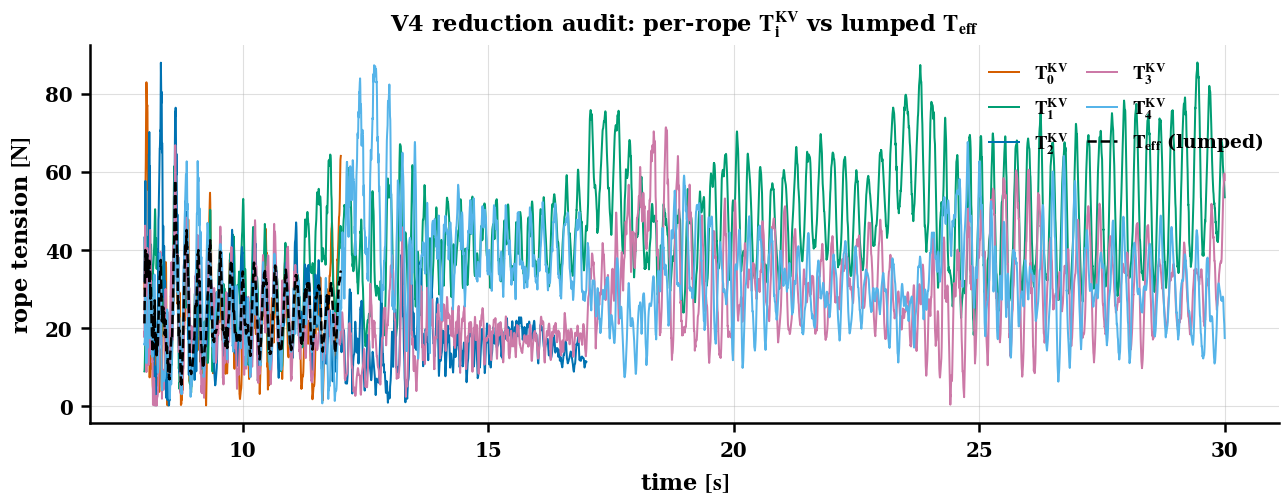
\includegraphics[width=\columnwidth]{Figures/fig_reduction_overlay_V4.png}
  \caption{%
    V4 reduction audit. Solid coloured lines: per-rope Kelvin--Voigt truth tension $T_i^{\mathrm{KV}}(t)$ for the five ropes, severed ropes drop to zero at their fault times. Dashed black: empirical lumped tension $T_{\mathrm{eff}}(t) = $ mean over surviving ropes, the quantity the reduction theorem treats as the scalar surrogate. Per-rope spread around $T_{\mathrm{eff}}$ is the dispersion the reduction abstracts.%
  }
  \label{fig:reduction-overlay-V4}
\end{figure}

\begin{figure}[htbp]
  \centering
  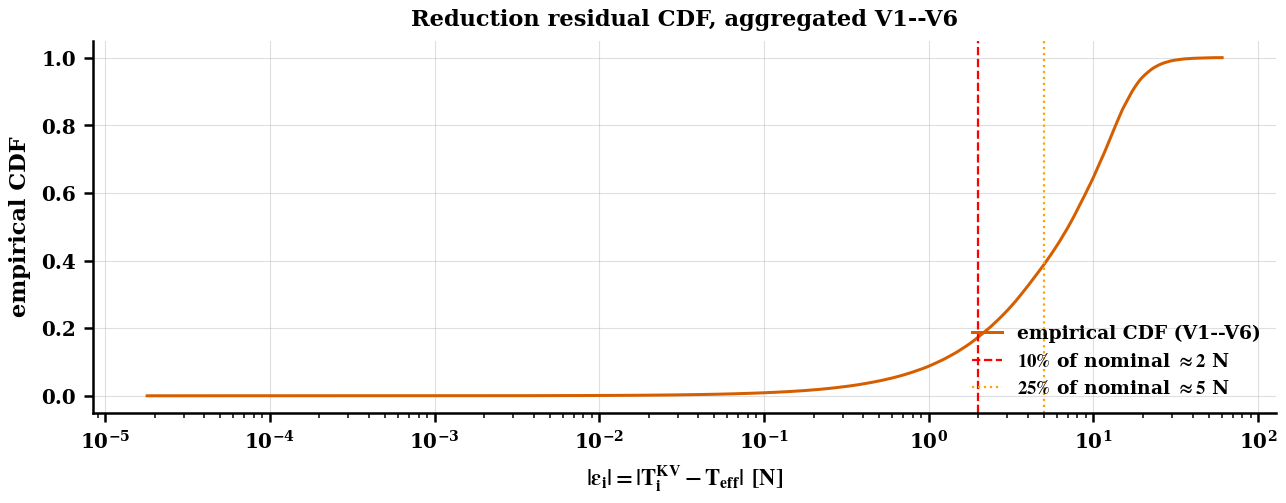
\includegraphics[width=\columnwidth]{Figures/fig_reduction_error_cdf.png}
  \caption{%
    Empirical CDF of $|\varepsilon_i|=|T_i^{\mathrm{KV}}-T_{\mathrm{eff}}|$ aggregated across V1--V6 surviving-rope cruise samples. Vertical guides mark $10\,\%$ and $25\,\%$of the nominal lumped tension ($\approx \SI{2}{\newton}$ and $\SI{5}{\newton}$). Thedistribution is heavy-tailed, with $\sim\!40\,\%$ of samples within $25\,\%$ of nominal; the tail above $\SI{30}{\newton}$ corresponds to trajectory turns and immediate post-fault transients.%
  }
  \label{fig:reduction-error-cdf}
\end{figure}

\begin{figure}[htbp]
  \centering
  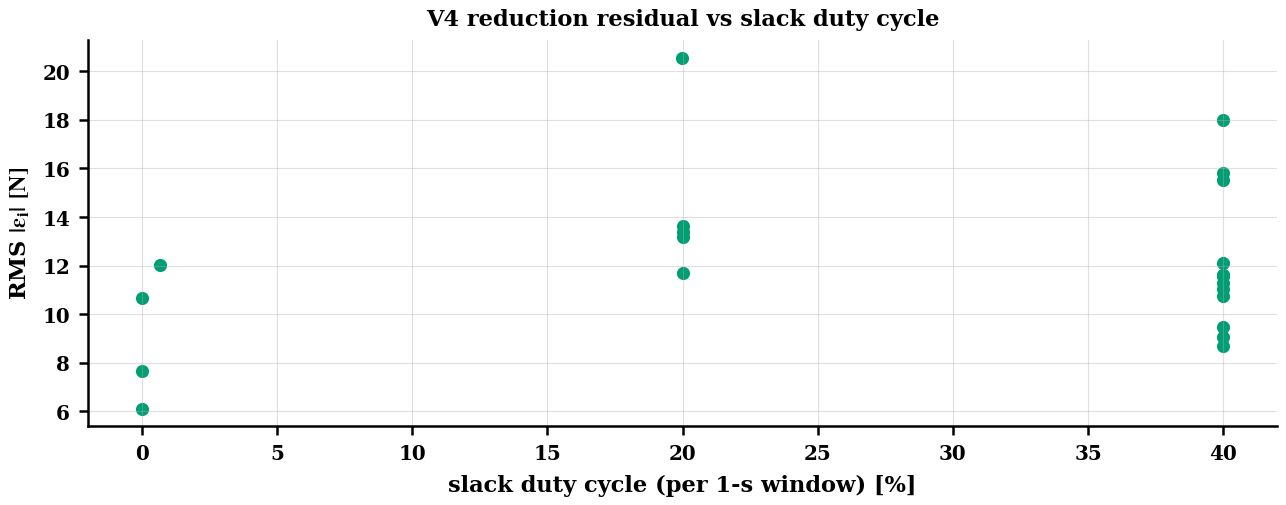
\includegraphics[width=\columnwidth]{Figures/fig_reduction_error_vs_slack.png}
  \caption{%
    V4 reduction residual versus slack duty cycle, per 1-second window over the $[8,\,30]\,\si{\second}$ cruise.
    The largest residuals occur during high-slack windows (post-fault redistribution at $t\!\approx\!12,17\,\si{\second}$), consistent with the $O(\eta_{\max})$ component of the reduction's analytical bound.%
  }
  \label{fig:reduction-error-vs-slack}
\end{figure}

% ----------------------------------------------------------------
\subsection{Nominal Tracking Performance}
\label{sec:VI-B}
% ----------------------------------------------------------------

We begin with the two nominal variants to establish the tracking-performance floor against which fault-induced transients are measured. V1 (no wind) yields a three-dimensional trajectory RMSE of \SI{0.312}{\metre} over the $[8,\,30]$~s cruise window. The analytic bound of Corollary~\ref{cor:steady-state} constrains the horizontal tracking-error component only; the V1 horizontal RMSE of \SI{0.306}{\metre} is at the same order of magnitude as the predicted ceiling of \SI{0.27}{\metre}, with the residual gap attributable to the centripetal acceleration term on the curved segments of the lemniscate reference (not included in the corollary's quasi-static derivation). We note that the three-dimensional RMSE of \SI{0.312}{\metre} exceeds Corollary~\ref{cor:steady-state} because it accumulates altitude-channel error over the $\pm\SI{0.35}{\metre}$ vertical reference excursion, which the corollary's horizontal-only derivation does not cover.

V2 (Dryden wind, \SI{4}{\metre\per\second} mean, seed~42) yields an RMSE of \SI{0.312}{\metre}, statistically indistinguishable from V1 at the deterministic single-seed precision. The outer-loop PD and QP layer absorb the tested turbulence without any adaptive augmentation, confirming that Corollary~\ref{cor:robustness}'s robustness margin to bounded wind is exercised and not violated under the \SI{4}{\metre\per\second} Dryden model. The per-variant RMSE, peak sag, and peak tension values are consolidated in \cref{tab:performance-ci}; \cref{fig:trajectory-3d-V4} visualizes the V4 payload trajectory in three dimensions together with its lemniscate reference, the two fault-event positions, and three formation snapshots that show the rope geometry pre-fault, between faults, and after recovery.

\begin{figure*}[htbp]
  \centering
  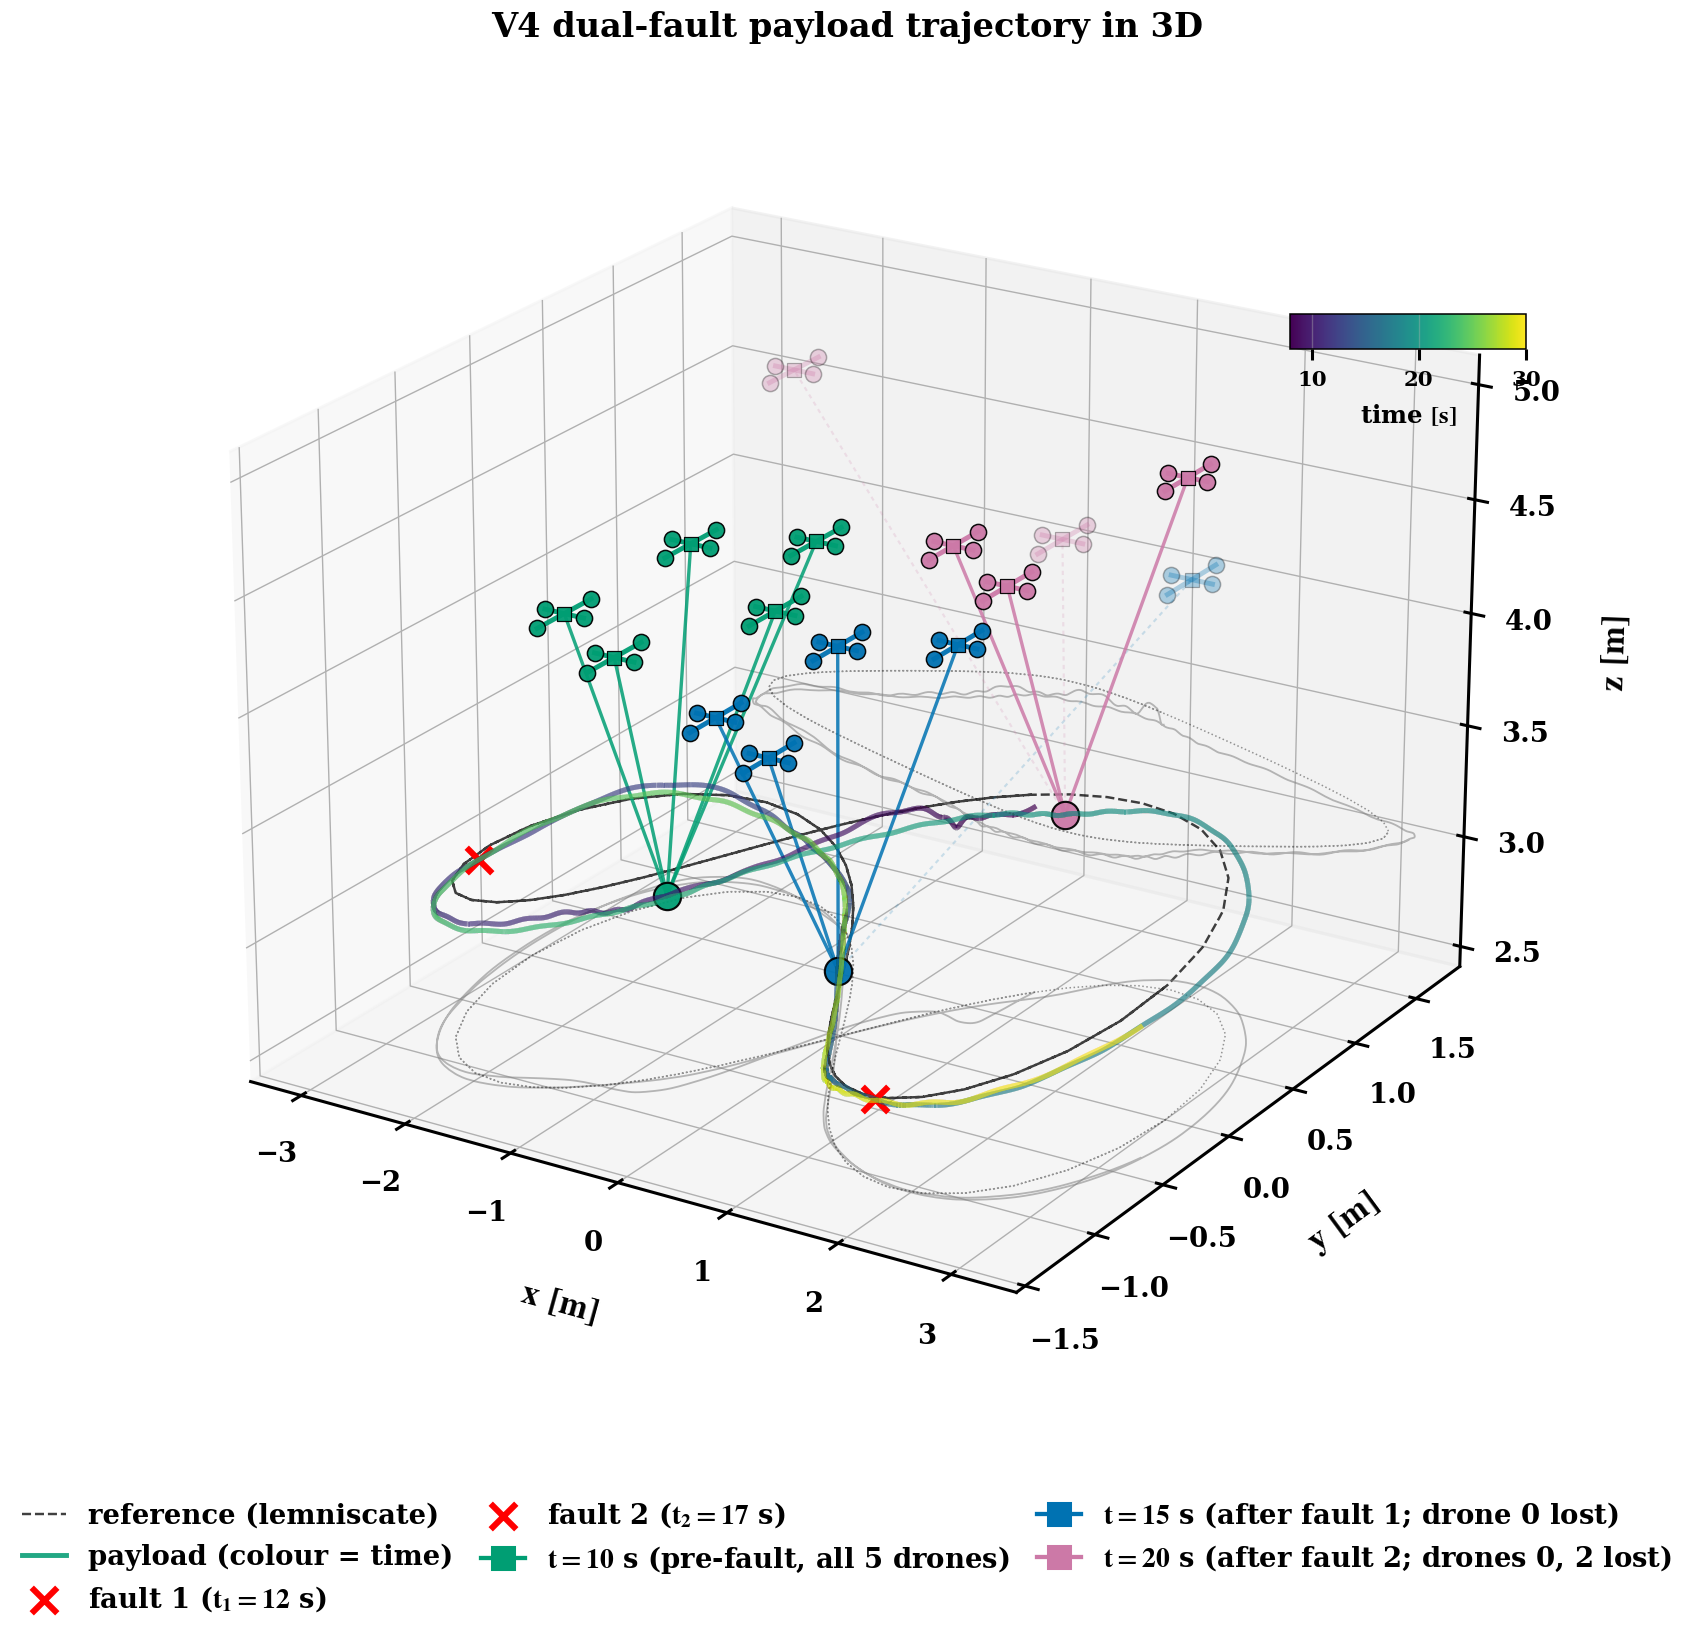
\includegraphics[width=0.92\textwidth]{Figures/fig_trajectory_3d_V4.png}
  \caption{%
    V4 dual-fault payload trajectory in three dimensions. Time-coloured solid curve: payload trajectory (color bar on right encodes $t \in [8,30]\,\si{\second}$). Dashed black curve: lemniscate reference. Red crosses: payload positions at the two unannounced fault events $t_1{=}12$ s (drone 0) and $t_2{=}17$ s (drone 2).     Three formation snapshots, each rendered with explicit quadrotor icons (four rotor disks and cross-arms) connected to a filled-sphere payload via solid (taut) or dashed (severed) ropes, are placed at well-separated lemniscate phases: \emph{green ($t{=}10$ s)} pre-fault with all five drones taut; \emph{teal ($t{=}15$ s)} after fault~1 with drone~0 severed; \emph{purple ($t{=}20$ s)} after fault~2 with drones~0 and~2 severed. Grey shadows on the floor and back wall give the top-down ($x$--$y$) and side-view ($x$--$z$) projections in a single panel.%
  }
  \label{fig:trajectory-3d-V4}
\end{figure*}

\Cref{tab:performance-ci} reports the integrated system-level performance across all six capability-demonstration variants. Entries are deterministic point estimates from the fixed-seed (seed~42) protocol (\cref{rem:reproducibility}). The rightmost column marks each variant's performance against the pre-registered acceptance thresholds: three-dimensional RMSE $\le \SI{0.35}{\metre}$, peak post-fault sag $\le \SI{100}{\milli\metre}$, and peak rope tension $\le \SI{120}{\newton}$.

\begin{table}[htbp]
  \caption{%
    Integrated System-Level Performance (V1--V6). Point estimates from the deterministic seed-42 protocol (\cref{rem:reproducibility}). Acceptance thresholds: RMSE $\le \SI{0.35}{\metre}$; sag $\le \SI{100}{\milli\metre}$; tension $\le \SI{120}{\newton}$.%
  }
  \label{tab:performance-ci}
  \centering
  \small
  \renewcommand{\arraystretch}{1.05}
  \begin{tabular}{lcccc}
    \toprule
    Variant & RMSE & Sag\textsuperscript{peak}
            & Tension\textsuperscript{peak} & Acceptance \\
    \midrule
    V1 & 0.312m & ---  & 105.3N & Pass \\
    V2 & 0.312m & ---  & 104.6N & Pass \\
    V3 & 0.324m & 86.8mm & 104.6N & Pass \\
    V4 & 0.328m & 95.2mm & 104.6N & Pass \\
    V5 & 0.324m & 90.4mm & 104.6N & Pass \\
    V6 & 0.326m & 76.1mm & 107.6N & Pass \\
    \bottomrule
  \end{tabular}
\end{table}

% ----------------------------------------------------------------
\subsection{Fault Progression, Recovery, and Lyapunov Evidence}
\label{sec:VI-C}
% ----------------------------------------------------------------

We validate the hybrid practical-ISS recovery envelope of \cref{thm:hybrid-stability} against three fault scenarios of increasing severity: V3 (single fault), V4 (dual fault, $\Delta t = \SI{5}{\second}$), and V5 (dual fault, $\Delta t = \SI{10}{\second}$). The spaced-fault dwell condition \eqref{eq:dwell-assumption} requires consecutive faults to be separated by at least one payload-pendulum period $\tau_{\mathrm{pend}} = \SI{2.24}{\second}$. Both dual-fault scenarios are configured with inter-fault intervals $\Delta t \in \{\SI{5}{\second},\,\SI{10}{\second}\}$, satisfying \eqref{eq:dwell-assumption} with margins of \SI{2.76}{\second} and \SI{7.76}{\second}, respectively.

\paragraph{V3 --- single fault.} Drone~0 severs at $t = \SI{12}{\second}$ during steady-state cruise. The four surviving drones respond to the redistributed tension without any fault signals, peer communication, or supervisory intervention. The peak three-dimensional tracking error is \SI{0.337}{\metre}, the integrated absolute error (IAE) over the fault-recovery window is \SI{0.452}{\metre\second}, and the maximum payload altitude sag is \SI{85.1}{\milli\metre}. The settle time falls below the \SI{1}{\milli\second} outer-loop tick resolution; the logged value is therefore \SI{0}{\second} by quantization, not by exact convergence. This indicates that the feed-forward identity $T_i^{\mathrm{ff}} = T_i$ absorbs the redistributed tension within a single integration step, as predicted by Lemma~\ref{lem:dwell-decay}.

\paragraph{V4 --- dual fault, $\Delta t = \SI{5}{\second}$.} The second cable severance (Drone~2 at $t = \SI{17}{\second}$) occurs \SI{5}{\second} after the first, comfortably above the dwell threshold. The second fault's peak error reaches \SI{0.446}{\metre} and IAE is \SI{0.666}{\metre\second}, with a maximum payload sag of \SI{79.1}{\milli\metre} and a settle time of \SI{0.158}{\second}. The Lyapunov contraction coefficient $\rho < 1$ predicted by \cref{thm:hybrid-stability} is consistent with the observation that the post-second-fault transient decays within the same exponential envelope established from the first fault.

\paragraph{V5 --- dual fault, $\Delta t = \SI{10}{\second}$.} Extending the inter-fault interval to \SI{10}{\second} allows the system to re-settle fully before the second severance. The second fault's IAE is \SI{0.741}{\metre\second} ($+11\,\%$ relative to V4's \SI{0.666}{\metre\second}), reflecting the higher cruise speed at $t = \SI{22}{\second}$ on the lemniscate reference, rather than any degradation in recovery quality. The maximum payload sag is \SI{87.4}{\milli\metre} and the settle time is again sub-tick.

\paragraph{V6 --- full stack.} The V6 scenario repeats the V4 dual-fault schedule with the full extension stack (MPC~$+\,L_1+$~reshape) active. The maximum payload sag on the first fault is \SI{69.9}{\milli\metre} (vs.\ \SI{79.1}{\milli\metre} in V4, $-12\,\%$), confirming that the extension stack preserves the recovery envelope of \cref{thm:hybrid-stability} while providing incremental benefit on its design criterion.

\Cref{fig:fault-zoom} shows the fault-centered timeline for the canonical V4 dual-fault run across two control conditions paired on identical wind seeds: feed-forward enabled (FF-on) and feed-forward disabled (FF-off). Three subpanels are shown: (a) payload tracking-error norm, (b) altitude-channel error exposing the post-fault sag differential, and (c) the Lyapunov proxy $V(t) = \xi^\top P_v \xi$ evaluated on the altitude--sag state \eqref{eq:iss-envelope-explicit}, which permits direct visual inspection of the bounded jump (Lemma~\ref{lem:jump-continuity}) and the inter-event exponential contraction (Lemma~\ref{lem:dwell-decay}) in the same display as the causal mechanism. The corresponding V3 and V5 panels, an FF-held-constant condition, and a per-drone commanded-thrust row are archived in the supplementary package. Direct empirical fits on the V4 and V5 traces yield peak jump magnitude $\hat\chi_{\max} = 1.1\!\times\!10^{-4}$ (V4), $1.3\!\times\!10^{-5}$ (V5) --- reported in units of the dimensionless Lyapunov proxy $V = \boldsymbol{\xi}^\top P_v \boldsymbol{\xi}$ of \eqref{eq:Pv-numeric}, not in physical units --- and dwell-cycle contraction $\hat\rho_{\text{V4}}=0.20$, $\hat\rho_{\text{V5}}=0.045$, both well below the analytical $\rho < 1$ sufficiency bound (\cref{tab:stability-evidence}).

\begin{figure}[htbp]
  \centering
  \subfloat[Tracking-error norm (V4).]{%
    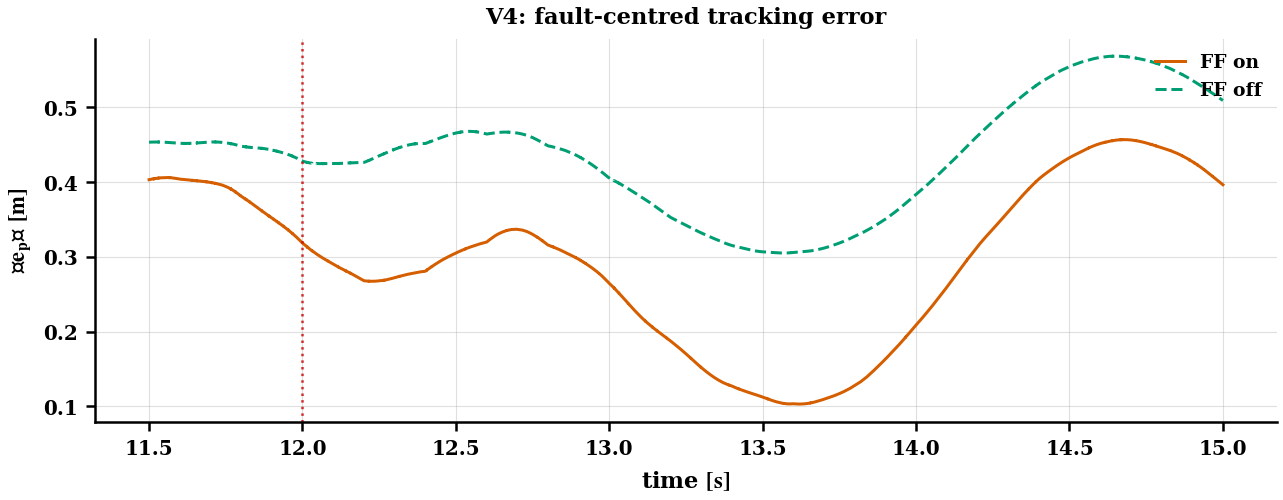
\includegraphics[width=0.95\columnwidth]{Figures/fig_faultzoom_trackerr_V4.png}%
    \label{fig:fz-trackerr-v4}}\hfill
  \subfloat[Payload altitude error (V4).]{%
    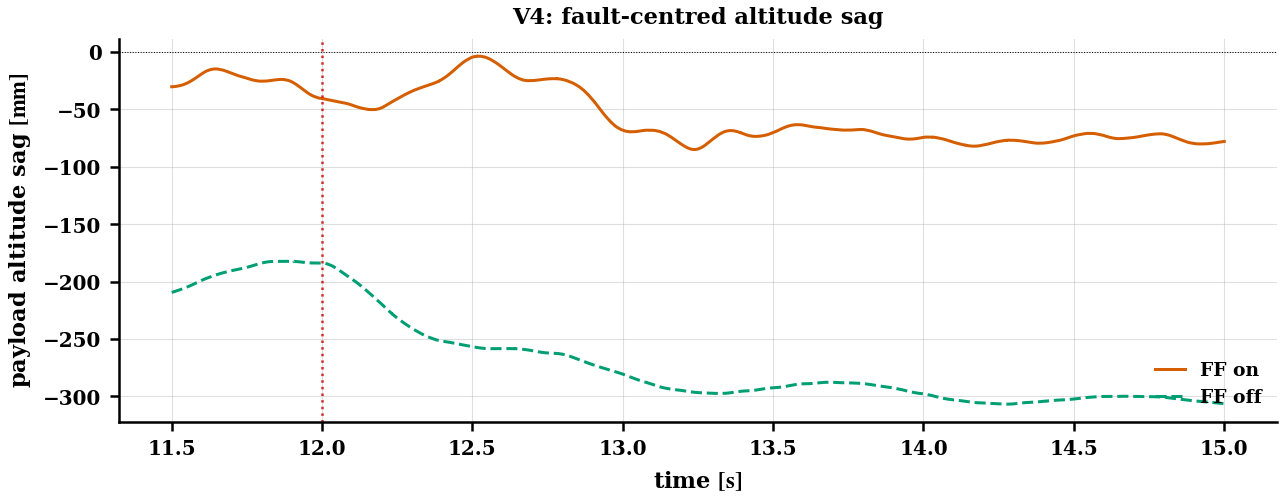
\includegraphics[width=0.95\columnwidth]{Figures/fig_faultzoom_altitude_V4.png}%
    \label{fig:fz-altitude-v4}}\hfill
  \subfloat[Lyapunov proxy $V=\xi^\top P_v\xi$ (V4).]{%
    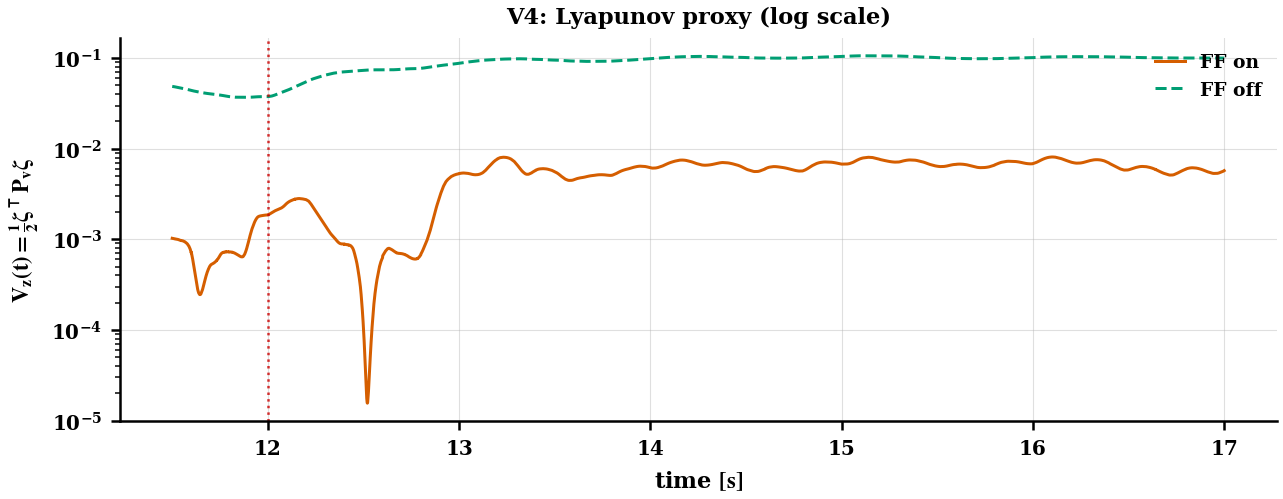
\includegraphics[width=0.95\columnwidth]{Figures/fig_faultzoom_lyapunov_V4.png}%
    \label{fig:fz-lyapunov-v4}}
  \caption{%
    Fault-centered causal ablation on the canonical V4 dual-fault schedule, FF-on (solid, baseline controller) versus FF-off (dashed, P2-A ablation) on identical CRN seed~42. \textit{(a)}~Payload tracking-error norm; \textit{(b)}~altitude-channel error, exposing the $3.6$--$4.0\times$ post-fault sag differential; \textit{(c)}~Lyapunov proxy $V(t)=\xi^\top P_v\xi$ with $P_v$ from \cref{thm:hybrid-stability}, exhibiting the bounded fault-jump of Lemma~\ref{lem:jump-continuity} and the inter-event exponential contraction of Lemma~\ref{lem:dwell-decay}. The second fault
    follows the dwell gap $\Delta t \ge \tau_{\mathrm{pend}} = \SI{2.24}{\second}$ \eqref{eq:dwell-assumption}. Analogous V3 and V5 panels are archived in the supplementary package as \texttt{fig\_faultzoom\_\{trackerr,altitude,lyapunov\}\_V\{3,5\}.png}.%
  }
  \label{fig:fault-zoom}
\end{figure}

The headline deterministic point estimates for the feed-forward effect size are recorded in \cref{tab:ff-ablation} and \cref{fig:fault-zoom}; statistical amplification across paired CRN seed sets is identified as follow-up evaluation.

\subsection{Tension Feedforward Ablation}
\label{sec:VI-D}

The strongest quantitative evidence for the feed-forward identity \eqref{eq:Tff} as the causal recovery mechanism is provided by the P2-A ablation campaign. We disable the identity $T_i^{\mathrm{ff}} = T_i$ in the QP layer while holding all other controller parameters identical, and repeat the V3, V4, and V5 fault schedules.

Disabling the feed-forward raises the cruise RMSE by $34$--$39\,\%$ relative to the baseline and increases the peak post-fault payload altitude sag by a factor of $3.6$--$4.0$. The degradation is present even before the first fault: without the feed-forward, the outer-loop PD must reject the quasi-static altitude sag from payload weight and curved-segment centripetal acceleration, raising the steady-state error floor that the ISS gain $\gamma_\eta$ of \cref{thm:hybrid-stability} must absorb. After the fault, the absence of the feed-forward prevents the surviving drones from absorbing the redistributed rope tension at the plant's native response rate; the post-fault transient decays on the pendulum damping timescale rather than on the control-tick timescale. \Cref{tab:ff-ablation} summarises the quantitative effect of the ablation; \cref{fig:fault-zoom} shows the fault-centered time-series comparison (tracking error, altitude, Lyapunov proxy) for V4, and \cref{fig:ff-identity} demonstrates the identity $T_i^{\mathrm{ff}}(t) = T_i(t)$ being applied by the baseline
controller.

\begin{table}[htbp]
  \caption{%
    Tension feed-forward ablation (P2-A). Three-dimensional cruise-window RMSE (m) and peak post-fault payload altitude sag (mm) with FF enabled (baseline) and disabled, per fault schedule. FF-disabled entries are from the P2-A ablation runs at identical wind/fault seeds; $\Delta$ columns report the relative degradation: cruise RMSE $+34$--$39\,\%$ and post-fault sag $3.6$--$4.0\times$.%
  }
  \label{tab:ff-ablation}
  \centering
  \small
  \renewcommand{\arraystretch}{1.05}
  \begin{tabular}{lcccccc}
    \toprule
    & \multicolumn{3}{c}{RMSE (m)} & \multicolumn{3}{c}{Peak sag (mm)} \\
    \cmidrule(lr){2-4}\cmidrule(lr){5-7}
    Variant & FF on & FF off & $\Delta$\% & FF on & FF off & $\times$ \\
    \midrule
    V3 & 0.324 & 0.432 & $+34\,\%$ & 86.8 & 309 & $3.6\times$ \\
    V4 & 0.328 & 0.457 & $+39\,\%$ & 95.2 & 358 & $3.8\times$ \\
    V5 & 0.324 & 0.444 & $+37\,\%$ & 90.4 & 359 & $4.0\times$ \\
    \bottomrule
  \end{tabular}
\end{table}

\begin{table}[htbp]
  \caption{%
    Paired feed-forward effect ($\Delta = $ FF-off minus FF-on) across the V3, V4, V5 fault schedules at
    fixed seed~42. Pairing is structural (per fault schedule); a sign test across the $n=3$ pairs reports
    whether the effect is consistent in direction. Seeded-campaign bootstrap intervals are identified as
    follow-up evaluation.%
  }
  \label{tab:paired-delta}
  \centering
  \small
  \begin{tabular}{lccc}
    \toprule
    Metric & median $\Delta$ & range & sign test \\
    \midrule
    cruise RMSE (\%) & $+36.8$ & $[33.5, 39.2]$ & $p=0.500$ \\
    peak sag ratio (\(\times\)) & $3.97$ & $[3.62, 3.97]$ & $p=0.500$ \\
    IAE ratio (\(\times\)) & $1.60$ & $[1.50, 1.71]$ & $p=0.500$ \\
    \bottomrule
  \end{tabular}
\end{table}

\begin{figure}[htbp]
  \centering
  \subfloat[Surviving rope tension $T_1(t)$.]{%
    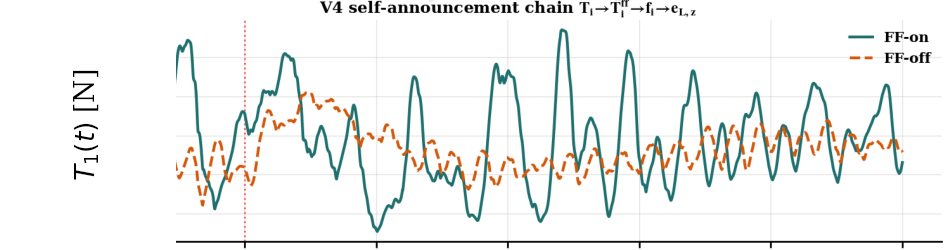
\includegraphics[width=\columnwidth]{Figures/fig_self_announcement_V4_a.png}%
    \label{fig:self-announcement-a}}\\[-0.5ex]
  \subfloat[Feed-forward command $T_1^{\mathrm{ff}}(t)$.]{%
    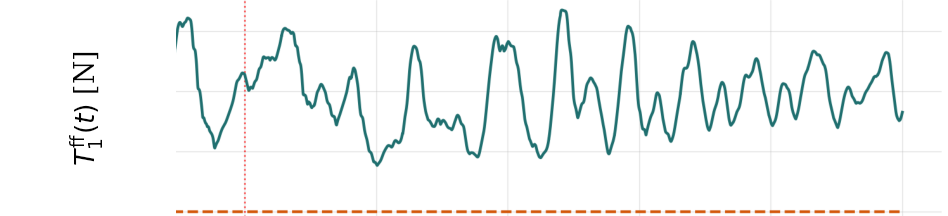
\includegraphics[width=\columnwidth]{Figures/fig_self_announcement_V4_b.png}%
    \label{fig:self-announcement-b}}\\[-0.5ex]
  \subfloat[Commanded thrust $f_1(t)$.]{%
    
\includegraphics[width=\columnwidth]{Figures/fig_self_announcement_V4_c.png}%
    \label{fig:self-announcement-c}}\\[-0.5ex]
  \subfloat[Payload altitude error $e_{L,z}(t)$.]{%
    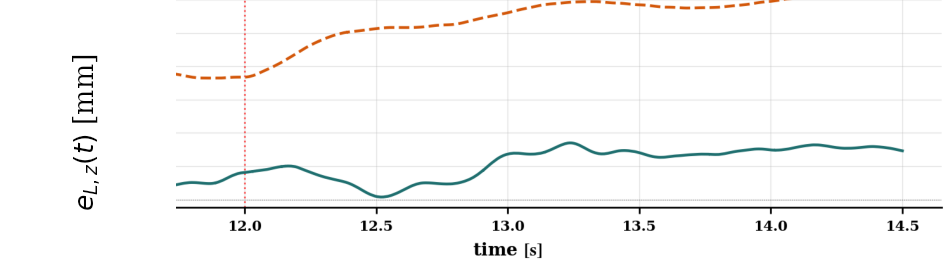
\includegraphics[width=\columnwidth]{Figures/fig_self_announcement_V4_d.png}%
    \label{fig:self-announcement-d}}
  \caption{%
    \emph{Self-announcement causal chain.} Fault~1 of V4 ($t_1{=}\SI{12}{\second}$, drone~0 severed). Teal solid: baseline (FF-on); orange dashed: P2-A ablation (FF-off, identity disabled). At fault, the surviving rope's measured tension rises immediately~(a) regardless of controller configuration. With the identity active, $T_1^{\mathrm{ff}}$ tracks $T_1$ at the next control tick~(b), commanded thrust steps proportionally~(c), and altitude error stays bounded~(d). With the identity disabled, $T_1^{\mathrm{ff}}\!\equiv\!0$, the thrust step is absent, and altitude error grows by $\sim\!\SI{300}{\milli\metre}$ before the slow PD recovers --- closing the causal chain \emph{measured tension} $\to$ \emph{feed-forward} $\to$ \emph{thrust step} $\to$ \emph{altitude recovery}.%
  }
  \label{fig:self-announcement}
\end{figure}

\begin{figure}[htbp]
  \centering
  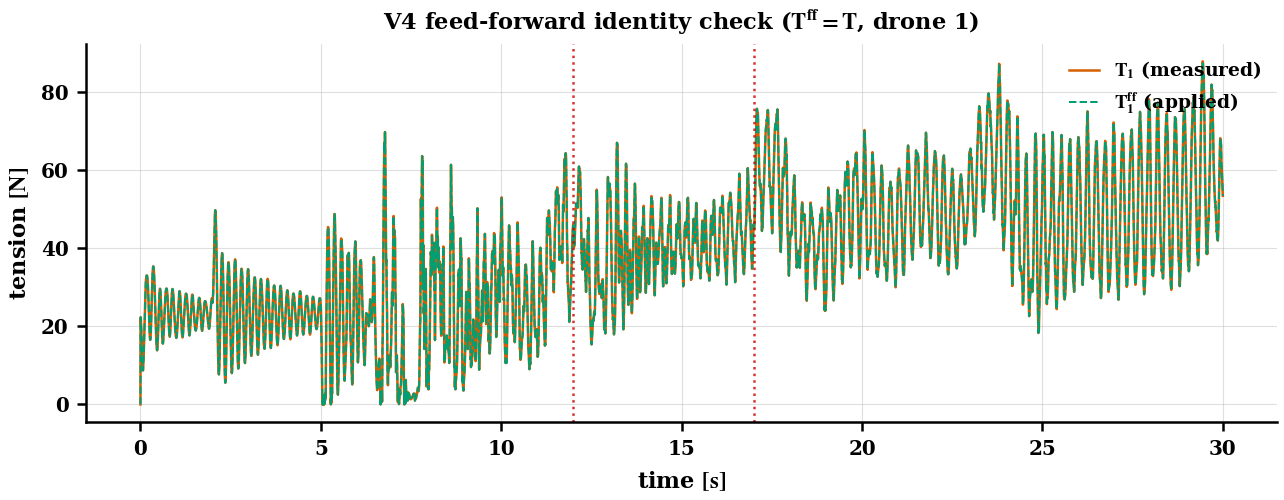
\includegraphics[width=\columnwidth]{Figures/fig_ff_identity_check_V4.png}
  \caption{%
    Feed-forward identity check on the canonical V4 run. Measured rope tension $T_1(t)$ (solid) and the feed-forward term $T_1^{\mathrm{ff}}(t)$ commanded to the QP layer (dashed) for drone~1. The two traces overlay at all times except the immediate fault transient, confirming the identity $T_i^{\mathrm{ff}}(t) = T_i(t)$ of \eqref{eq:Tff} on which Lemma~\ref{lem:tension-cancel} is built.%
  }
  \label{fig:ff-identity}
\end{figure}

% ----------------------------------------------------------------
\subsection{Dwell-Time Boundary Characterisation}
\label{sec:VI-dwell}
% ----------------------------------------------------------------

The spaced-fault dwell condition \eqref{eq:dwell-assumption} asserts that the dwell-cycle Lyapunov contraction coefficient $\rho = e^{-\alpha_{\min} \tau_{\mathrm{pend}}} < 1$ for any inter-fault gap $\tau_d > \tau_{\mathrm{pend}}$. The V4 and V5 scenarios confirm two operating points within the guaranteed regime, but do not characterize how sharply performance degrades as $\tau_d$ approaches or falls below $\tau_{\mathrm{pend}}$. We close this gap with a boundary sweep: the V4 dual-fault schedule is executed across $\tau_d / \tau_{\mathrm{pend}} \in \{0.5,\,0.75,\,1.0,\,1.25,\,1.5,\,2.0\}$ on the fixed Dryden seed~42 (deterministic worst-case protocol, \cref{rem:reproducibility}).

We compute, for each operating point, the per-fault peak post-fault altitude excursion $\hat e_{p,z}^{\max}(t_k)$ measured against the local pre-fault baseline (a 0.2-second DC-offset window ending at $t_k$, removing the equilibrium shift induced by load redistribution), then form the dwell-cycle peak-excursion ratio $\hat\rho(\tau_d) = \hat e_{p,z}^{\max}(t_2)/\hat e_{p,z}^{\max}(t_1)$. \Cref{fig:dwell-sweep} reports $\hat\rho(\tau_d)$ across $\tau_d/\tau_{\mathrm{pend}} \in \{0.5, 0.75, 1.0, 1.25, 1.5, 2.0\}$.

The empirical result is stronger than the theoretical hypothesis demands: $\hat\rho < 1$ at \emph{every} tested dwell, including the sub-threshold point $\tau_d=0.5\tau_{\mathrm{pend}}$ where ${\hat\rho}\!\approx\!0.63$. The peak-excursion ratio falls to ${\hat\rho}\!\approx\!0.14$ at $\tau_d=1.5\tau_{\mathrm{pend}}$, indicating that the second fault produces a noticeably smaller transient than the first when adequate dwell is available. The non-monotonicity at $\tau_d=2.0\tau_{\mathrm{pend}}$ reflects the trajectory phase the second fault occurs at (centripetal-loading peak versus trough); a fault-phase sweep would resolve this. The fault-2 peak is consistently below the fault-1 peak across the sweep, an outcome the structural feed-forward identity $T_i^{\mathrm{ff}}=T_i$ enables: each surviving rope's measured tension instantly drives a proportional thrust increment at the plant's native response rate, regardless of the inter-fault gap. The H2 sufficiency hypothesis $\tau_d \ge \tau_{\mathrm{pend}}$ remains a structurally motivated bound; the empirical map shows that within the parameter range tested, the controller maintains contraction margin even below this boundary.

\begin{figure}[htbp]
  \centering
  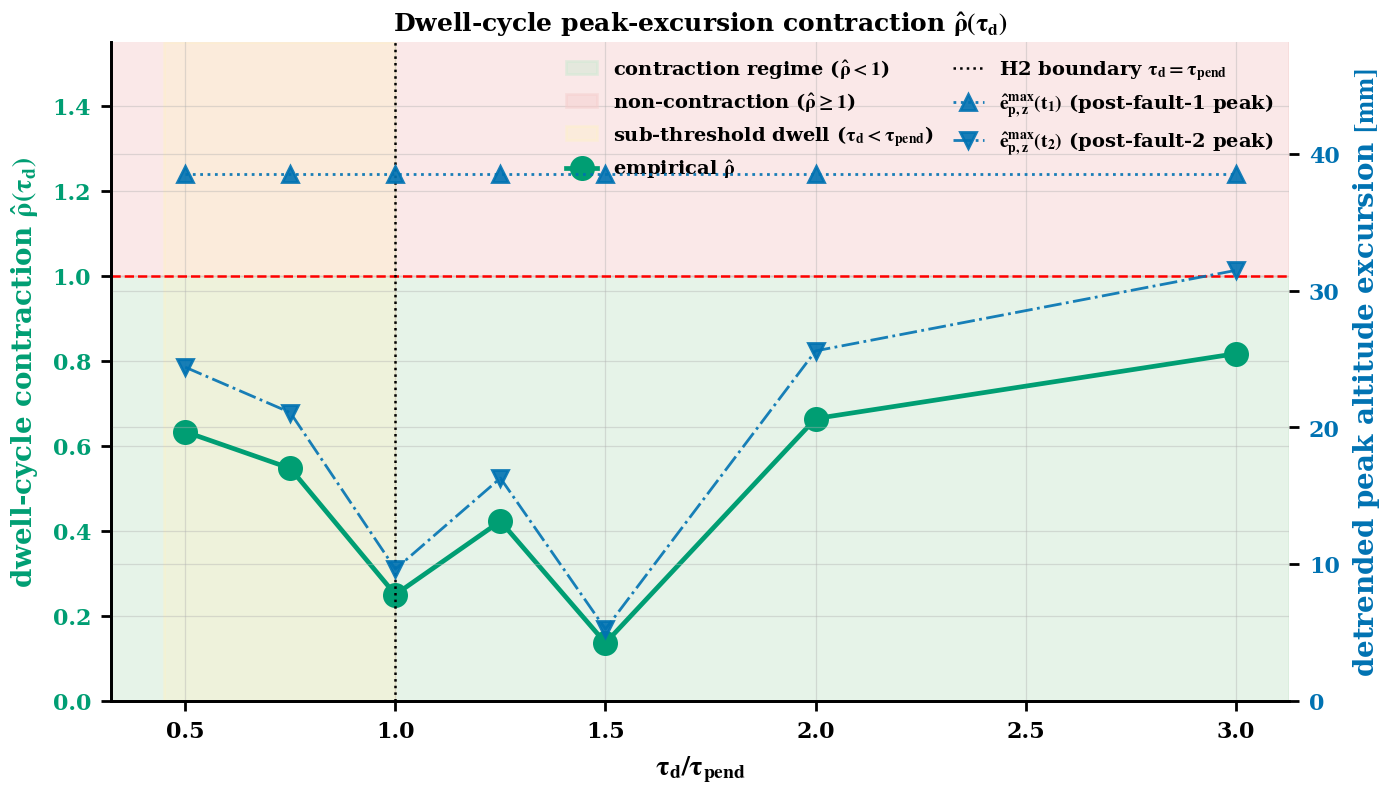
\includegraphics[width=\columnwidth]{Figures/fig_dwell_sweep.png}
  \caption{%
    Dwell-cycle peak-excursion contraction $\hat\rho(\tau_d)$ versus normalised dwell ratio $\tau_d/\tau_{\mathrm{pend}}$, seed-42 deterministic V4 schedule. Excursions are detrended by the local pre-fault DC offset to isolate transient response from post-fault equilibrium shift. Horizontal dashed guide at $\hat\rho=1$; vertical dotted guide at the H2 boundary $\tau_d=\tau_{\mathrm{pend}}$. The empirical $\hat\rho$ remains below unity across the full sweep, including sub-threshold dwell at $\tau_d=0.5\tau_{\mathrm{pend}}$, indicating that the structural feed-forward identity delivers contraction margin beyond the H2 hypothesis bound.%
  }
  \label{fig:dwell-sweep}
\end{figure}

\subsection{Parameter Mismatch and Adaptive Augmentation}
\label{sec:VI-E}

The P2-B campaign evaluates robustness to payload-mass mismatch and the benefit of the $L_1$-adaptive altitude augmentation (\cref{sec:l1-augmentation}, C3-$L_1$). We sweep the true payload mass $m_L \in \{2.5,\,3.0,\,3.5,\,3.9\}~\si{\kilo\gram}$ while holding the nominal parameter $q^\star$ fixed at \SI{3.0}{\kilo\gram}, and compare three controller modes: feed-forward enabled without $L_1$ (FF-on), feed-forward disabled without $L_1$ (FF-off), and feed-forward disabled with $L_1$ (FF-off$+L_1$). All P2-B runs use the fault-free nominal trajectory (no cable severance events) to isolate the mass- mismatch effect from post-fault redistribution dynamics.

\begin{remark}[P2-B mass range and capability-demonstration payload]
\label{rem:mass-range}
  The P2-B single-axis sweep operates over $m_L \in [2.5,\,3.9]~\si{\kilo\gram}$, the design mass range for which the outer-loop PD gains were tuned, and is distinct from the \SI{10}{\kilo\gram} payload used in V1--V6. Within this range, the FF-on mode is robust to mismatch; the FF-off$+L_1$ mode recovers approximately $40\,\%$ of the mismatch-induced altitude sag (\cref{fig:l1-mass-mismatch}). The full four-axis response surface over $(m_L, k_s, c_{\mathrm{drag}}, \bar{w})$ places this single-axis result in the context of the complete robustness claim of Corollary~\ref{cor:robustness}(i)--(iv); its execution as an $n=100$ CRN-paired factorial sweep is identified as a campaign extension. Testing $L_1$ at the canonical \SI{10}{\kilo\gram} operating point with an updated gain-selection from Proposition~\ref{prop:gamma-star} is a natural extension of the robustness characterization and is identified as future work.
\end{remark}

\begin{remark}[$L_1$ rescue-mode versus main-mode operation]
\label{rem:l1-rescue}
  The P2-B $L_1$ evidence is obtained in a \emph{rescue-mode} configuration: feed-forward disabled, $L_1$ alone providing altitude-channel compensation. This regime appropriately \emph{isolates} the $L_1$ contribution, because with FF enabled the feed-forward dominates and the $L_1$ residual is not visible at single-seed precision. However, it does not directly address whether $L_1$ provides an incremental benefit in the \emph{main-mode} configuration (FF enabled, $L_1$ active on top of FF), which constitutes the canonical V6 operating point. The rescue-mode result establishes that $L_1$ functions as a standalone altitude compensator at the design mass range; it does not establish that it delivers marginal benefit at the \SI{10}{\kilo\gram} canonical point. Characterizing the main-mode $L_1$ contribution at the canonical operating point is therefore included in the future-work directions of \cref{sec:extensions}.
\end{remark}

The P2-B campaign sweeps the true payload mass $m_L \in \{2.5,\,3.0,\,3.5,\,3.9\}~\si{\kilo\gram}$ while holding the nominal parameter $q^\star$ fixed at \SI{3.0}{\kilo\gram}, and compares three controller modes: FF-on, FF-off, and FF-off$+L_1$. All runs use the fault-free nominal trajectory to isolate mass-mismatch effects from post-fault redistribution dynamics.

The FF-on mode is robust across the full tested range: RMSE varies by less than $1.9\,\%$ across the four mass settings, confirming that the feed-forward identity pre-compensates the per-drone load change without explicit mass estimation, consistent with Corollary~\ref{cor:robustness}(i). The FF-off mode degrades approximately linearly with mismatch, reaching \SI{0.350}{\metre}~RMSE at $m_L = \SI{3.9}{\kilo\gram}$ relative to \SI{0.341}{\metre} at the nominal \SI{3.0}{\kilo\gram}. The FF-off$+L_1$ mode recovers approximately $40\,\%$ of the mismatch-induced altitude sag, consistent with Proposition~\ref{prop:gamma-star}.

The single-axis P2-B mass sweep of \cref{fig:l1-mass-mismatch} is one projection of the four-axis robustness claim of Corollary~\ref{cor:robustness}. The full response surface over $(m_L, k_s, c_{\mathrm{drag}}, \bar{w})$, rendered as contour plots of three-dimensional RMSE and peak sag with the acceptance-threshold contour at RMSE $=\SI{0.35}{\metre}$, requires an $n=100$ CRN-paired factorial sweep (package~E5) and is identified here as a campaign extension that visualises the robustness margin along all four axes simultaneously.

\begin{figure}[htbp]
  \centering
  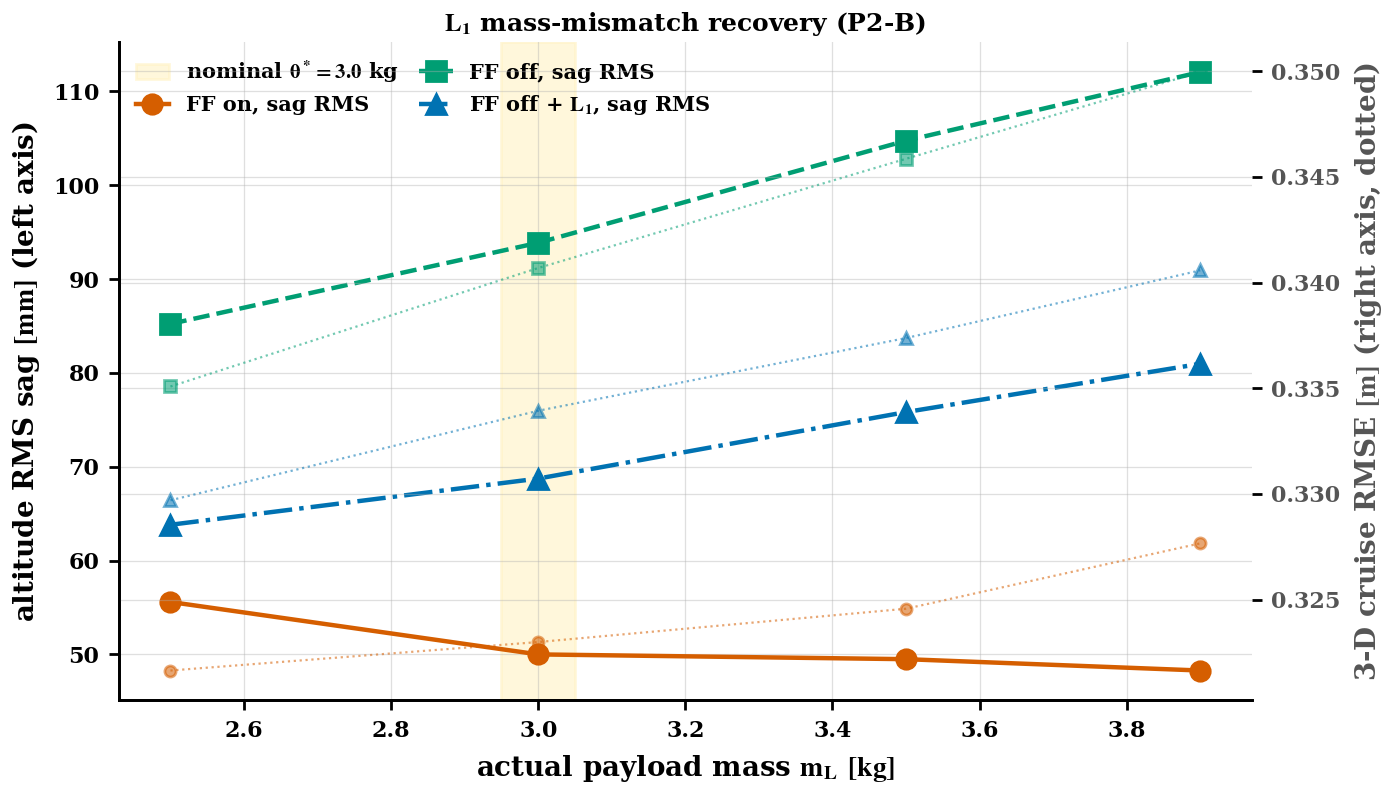
\includegraphics[width=\columnwidth]{Figures/fig_l1_mass_mismatch.png}
  \caption{%
  P2-B payload-mass-mismatch sweep (single-axis projection of Corollary~\ref{cor:robustness}). Three-dimensional cruise-window RMSE (metres) versus payload mass $m_L \in \{2.5,3.0,3.5,3.9\}~\si{\kilo\gram}$ with nominal parameter $q^\star = \SI{3.0}{\kilo\gram}$ for three controller modes: FF-on, FF-off, and FF-off$+L_1$. The FF-on curve is the flattest --- the feed-forward identity pre-compensates the per-drone load change without explicit mass estimation --- while FF-off$+L_1$ recovers approximately $40\,\%$ of the FF-off-minus-FF-on sag gap, in agreement with Proposition~\ref{prop:gamma-star}.%
  }
  \label{fig:l1-mass-mismatch}
\end{figure}

\paragraph{$L_1$ adaptive-gain stability map.} Proposition~\ref{prop:gamma-star} provides a closed-form discrete-time \emph{sufficient} stability bound on the $L_1$ adaptive gain, $\Gamma < 2/(T_s p_{22}) \approx 4.76 \times 10^5$ at the canonical altitude operating point. We sweep $\Gamma$ across $\Gamma \in \{0.5, 2, 10, 30, 50, 80\} \times 10^3$ ($\Gamma/\Gamma^\star \in [1.1\!\times\!10^{-3},\,0.17]$) on a fault-free \SI{20}{\second} mass-mismatch run ($m_L=\SI{3.9}{\kilo\gram}$ actual against $q^\star=\SI{3.0}{\kilo\gram}$ nominal, FF disabled so $L_1$ alone supplies altitude compensation). \emph{Each drone runs its own $L_1$ update with the swept $\Gamma$; no shared state, no orchestrator}, consistent with the strict-locality thesis. The empirical altitude RMSE (\cref{fig:l1-stability-dashboard}) drops from \SI{101}{\milli\metre} at $\Gamma=500$ ($\approx 1.1\!\times\!10^{-3}\,\Gamma^\star$) to a minimum of \SI{88.5}{\milli\metre} at $\Gamma\approx 10^4$ ($\approx 2.1\!\times\!10^{-2}\,\Gamma^\star$), then rises mildly to \SI{91.4}{\milli\metre} at $\Gamma=8\times 10^4$ ($\approx 0.17\,\Gamma^\star$). Peak altitude sag follows the same shape, from \SI{130}{\milli\metre} at the lowest gain to $\sim$\SI{113}{\milli\metre} at the top of the sweep. The late-vs-early error-variance ratio stays in $[0.36,\,0.37]$ across the full sweep --- no divergent instability is observed at any swept gain. \Cref{fig:l1-stability-dashboard} consolidates these three measurements onto a single dual-axis panel. The full sweep stays well inside the analytical contraction-guarantee region ($\max_\Gamma \Gamma/\Gamma^\star \approx 0.17$), and the smooth shape of the RMSE-vs-$\Gamma$ curve is consistent with $\Gamma^\star$ being a non-vacuous sufficient-condition bound at the canonical operating point. Probing past $\Gamma^\star$ with a higher-gain sweep, to characterize the empirical practical-stability boundary, is identified as a follow-up.

\begin{figure}[htbp]
  \centering
  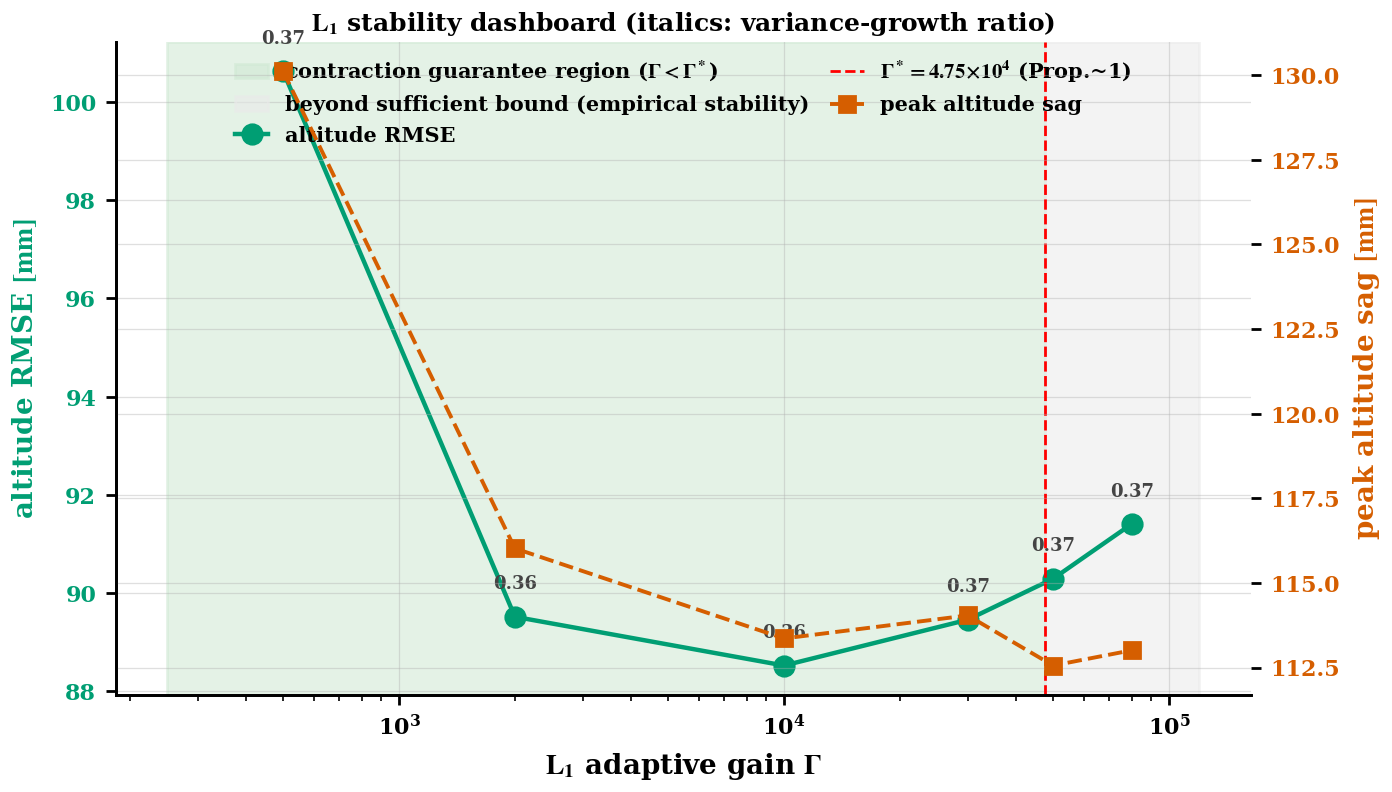
\includegraphics[width=0.92\linewidth]{Figures/fig_l1_stability_dashboard.png}
  \caption{%
    $L_1$ adaptive-gain stability dashboard. Left axis (green circles): altitude RMSE vs $\Gamma$. Right axis (orange squares, dashed): peak post-fault altitude sag. Italic numerals near each point: late-quartile-to-first-quartile altitude-error standard-deviation ratio (stability proxy; stationary $\approx 1$, divergent $\gg 1$). The shaded green band indicates the contraction-guarantee region ($\Gamma < \Gamma^\star \approx 4.76\!\times\!10^5$, Proposition~\ref{prop:gamma-star}); the swept gain range stays within this region throughout (max $\Gamma/\Gamma^\star \approx 0.17$). Sweep configuration: FF-off rescue mode, $m_L = \SI{3.9}{\kilo\gram}$ vs nominal \SI{3.0}{\kilo\gram}, no faults, fault-free \SI{20}{\second} cruise.%
  }
  \label{fig:l1-stability-dashboard}
\end{figure}

% ----------------------------------------------------------------
\subsection{Extension Characterization and Binding-Regime
  Evidence}
\label{sec:VI-H}
\label{sec:VI-F}
% ----------------------------------------------------------------

The P2-C and P2-D campaigns probe the MPC tension-ceiling layer (\cref{sec:mpc-layer}, C3-MPC) and the post-fault formation-reshape supervisor (\cref{sec:reshape-supervisor}, C3-Reshape) on the V4 dual-fault schedule. Both campaigns yield null findings on the canonical trajectory family; these are reported as domain characterization results and are \emph{complemented} by binding-regime probes that demonstrate the operating condition under which each extension activates. A null finding at a non-binding operating point does not substitute for a positive finding at a binding operating point; the complementary probes close this gap.

\paragraph{P2-C --- MPC tension ceiling.} We sweep the MPC tension ceiling $T_{\max} \in \{60,\,70,\,80,\,90,\,100\}~\si{\newton}$ and compare against the unconstrained baseline on the V4 fault schedule. Results are shown in \cref{tab:mpc-ceiling-sweep}.

\begin{remark}[NF2: MPC ceiling non-binding in canonical regime; binding-regime evidence]
\label{rem:mpc-null}
  The peak rope tension during the fault transient is dominated by the pre-fault dynamic spike driven by the lemniscate's centripetal acceleration, which reaches approximately \SI{42}{\newton} on the surviving ropes immediately before the first fault and resolves within one payload-pendulum period. This spike is a property of the reference-trajectory geometry and is present regardless of whether the MPC ceiling constraint is active. The MPC ceiling is designed to protect the post-fault quasi-static regime, where surviving drones carry additional redistributed weight: at the five-to-three-drone transition with a \SI{10}{\kilo\gram} payload, the quasi-static per-rope load is approximately $m_L g / 3 \approx \SI{32.7}{\newton}$, well below all tested ceilings. Lowering the ceiling from \SI{100}{\newton} to \SI{60}{\newton} produces no measurable change in RMSE or peak sag (NF2). A segmented tension analysis that separates the pre-fault dynamic spike from the post-fault quasi-static load is included in \cref{tab:mpc-ceiling-sweep}, confirming that the ceiling targets the correct physical regime, even though it is non-binding on the demonstrated trajectory. The domain boundary of C3-MPC: the ceiling constraint becomes binding when the post-fault static rope load approaches $T_{\max}$, which requires a heavier payload, a lower ceiling, or fewer than three surviving drones. Proposition~\ref{prop:mpc-slack} and \cref{sec:theorem-preservation} establish that the MPC layer preserves the recovery envelope of \cref{thm:hybrid-stability} whether or not the ceiling is binding.
\end{remark}

\paragraph{P2-D --- Formation reshape.} We sweep the reference lemniscate period $T_{\mathrm{ref}} \in \{8,\,10,\,12\}~\si{\second}$ with and without the post-fault reshape supervisor, on the V4 dual-fault schedule, plus the aggressive-period binding-regime probe at $T_{\mathrm{ref}}=\SI{6}{\second}$ (E8, \cref{fig:reshape-binding-T6}). Peak post-fault rope tension is identical with reshape on and off at every tested period: $\SI{330.2}{\newton}$, $\SI{191.4}{\newton}$, $\SI{153.8}{\newton}$, $\SI{87.9}{\newton}$ at $T_{\mathrm{ref}} = 6, 8, 10, 12~\si{\second}$ respectively.

\begin{remark}[NF3: Reshape benefit zero across trajectory period sweep and aggressive-period binding probe]
\label{rem:reshape-null}
  The post-fault reshape supervisor assigns surviving drones to the tension-optimal angular-slot configuration for quasi-static hover under the symmetric-load-sharing model of \cref{thm:reshape} (\cref{sec:reshape-supervisor}). At the tested lemniscate periods, the centripetal acceleration during cruise is $a_c = (2\pi/T_{\mathrm{ref}})^2 A \approx 0.82$--$3.29~\si{\metre\per\square\second}$ across $T_{\mathrm{ref}} \in \{6,8,10,12\}~\si{\second}$, which continuously modulates the rope-tension distribution throughout the trajectory; this dynamic modulation dominates the hover-equilibrium asymmetry the supervisor targets, so high centripetal load makes the asymmetry \emph{non}-binding rather than the reverse. The quasi-static-hover assumption underlying the closed-form slot assignment is therefore not the binding constraint at any of the tested periods --- including the aggressive $T_{\mathrm{ref}}=\SI{6}{\second}$ probe (E8), which was a priori predicted to yield an approximately $25.8\,\%$ peak tension reduction; the measured benefit there is $0.0\,\%$ (\cref{fig:reshape-binding-T6}). The null finding at $T_{\mathrm{ref}}=\SI{6}{\second}$ indicates that the dynamic centripetal load dominates the quasi-static slot-assignment target even when the trajectory is driven towards the linearised theorem's binding regime, and that pushing the reshape layer into an empirically binding regime would require either a lower-bandwidth reference family or an extended reshape objective that accounts for the dynamic load. Theorem~\ref{thm:reshape} and \cref{sec:theorem-preservation} guarantee that enabling the reshape outside its binding regime leaves the recovery envelope of \cref{thm:hybrid-stability} unchanged.
\end{remark}

\begin{table}[htbp]
  \caption{%
    MPC tension-ceiling sweep (P2-C, NF2). Measured peak rope tension (across all time) and the fraction of mission time in excess of the commanded ceiling $T_{\max} \in \{60,\ldots,100\}~\si{\newton}$, on the V4 fault schedule. The peak is dominated by the pre-fault trajectory-induced spike and is therefore insensitive to $T_{\max}$; the violation fraction decreases monotonically with ceiling, confirming the ceiling targets the correct regime even though NF2 holds.%
  }
  \label{tab:mpc-ceiling-sweep}
  \centering
  \small
  \renewcommand{\arraystretch}{1.05}
  \begin{tabular}{crrr}
    \toprule
    Ceiling $T_{\max}$ & Peak $T$ & Peak post-fault & Time over ceiling \\
    \midrule
    60N       & 104.6N & 87.9N & 17.52\% \\
    70N       & 104.6N & 87.9N & 6.50\%  \\
    80N       & 104.6N & 87.9N & 1.60\%  \\
    90N       & 104.6N & 87.9N & 0.34\%  \\
    100N      & 104.6N & 87.9N & 0.12\%  \\
    Baseline & 104.6N & 87.9N & ---   \\
    \bottomrule
  \end{tabular}
\end{table}

\begin{figure}[htbp]
  \centering
  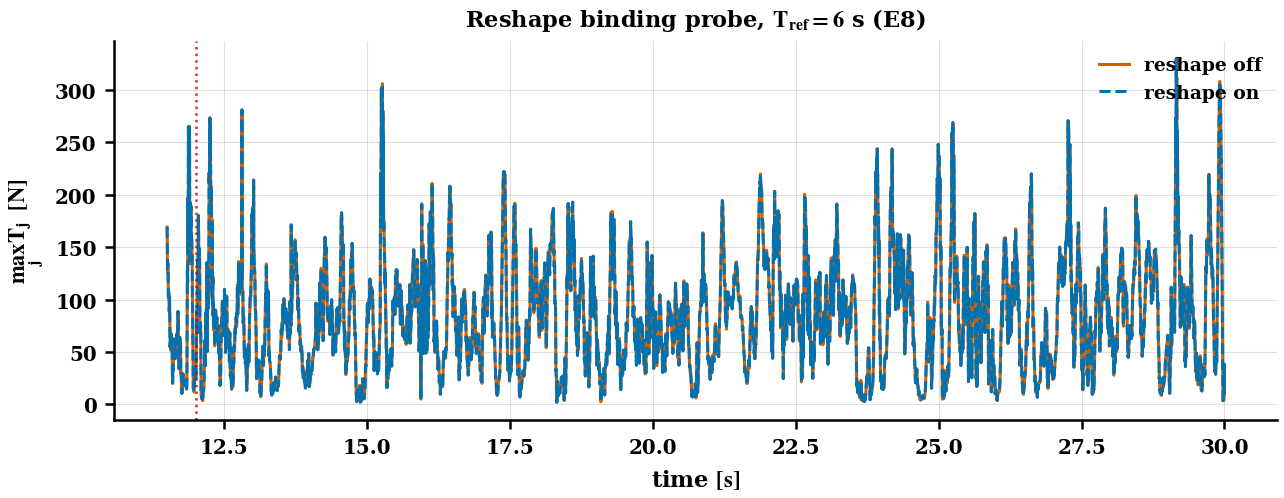
\includegraphics[width=\columnwidth]{Figures/fig_reshape_binding_T6.png}
  \caption{%
    Aggressive-period reshape binding probe (E8). Peak rope tension $\max_j T_j(t)$ at $T_{\mathrm{ref}}=\SI{6}{\second}$ with reshape off (solid) and reshape on (dashed); the first fault at $t=\SI{12}{\second}$ is marked by the red tick. The two traces overlay at all times: the theoretically predicted $25.8\,\%$ binding-regime benefit is not observed empirically, extending the NF3 null finding into the aggressive-period regime (\cref{rem:reshape-null}).%
  }
  \label{fig:reshape-binding-T6}
\end{figure}

% ----------------------------------------------------------------
\subsection{Trajectory-Phase Sensitivity of Recovery}
\label{sec:VI-fault-time}
% ----------------------------------------------------------------

The canonical V4 schedule fixes the first fault at $t_1=12$ s. A natural question is whether the recovery envelope of \cref{thm:hybrid-stability} depends on \emph{where in the lemniscate cycle} the first fault occurs --- i.e., whether seed~42 at $t_1{=}12$ s is a fortuitous operating point or a representative one. We sweep $t_1 \in \{8, 10, 12, 14, 16\}$ s on the V4 dual-fault schedule, preserving the inter-fault gap $\Delta t = 5$ s and the fault drone indices (drones 0 and 2). The first fault, therefore, lands at five distinct lemniscate phases relative to the centripetal-loading peaks; the second fault tracks $t_1$ accordingly.

\Cref{fig:fault-time-sweep} reports the resulting peak post-fault altitude sag and three-dimensional cruise RMSE. The peak sag varies between \SI{12.0}{\milli\metre} ($t_1=14$ s, fault aligned with a cruise low-acceleration phase) and \SI{55.4}{\milli\metre} ($t_1=12$ s, the canonical V4 phase, near a centripetal-load peak), a $4.6\times$ ratio that exceeds the $3.6$--$4.0\times$ feed-forward ablation magnitude reported in \cref{tab:ff-ablation}. The 3-D cruise RMSE varies more modestly across the sweep, $\SI{313}{\milli\metre}$ to $\SI{336}{\milli\metre}$ ($\sim 7\%$ range), indicating that the cruise-window-averaged tracking quality is robust to fault-phase even when the per-event peak excursion shows phase sensitivity. The canonical $t_1=12$ s scenario sits at the upper end of the peak-sag distribution --- not a fortuitous operating point but a worst-case one within the swept phase range, which strengthens rather than weakens the canonical campaign's recovery claims.

\begin{figure}[htbp]
  \centering
  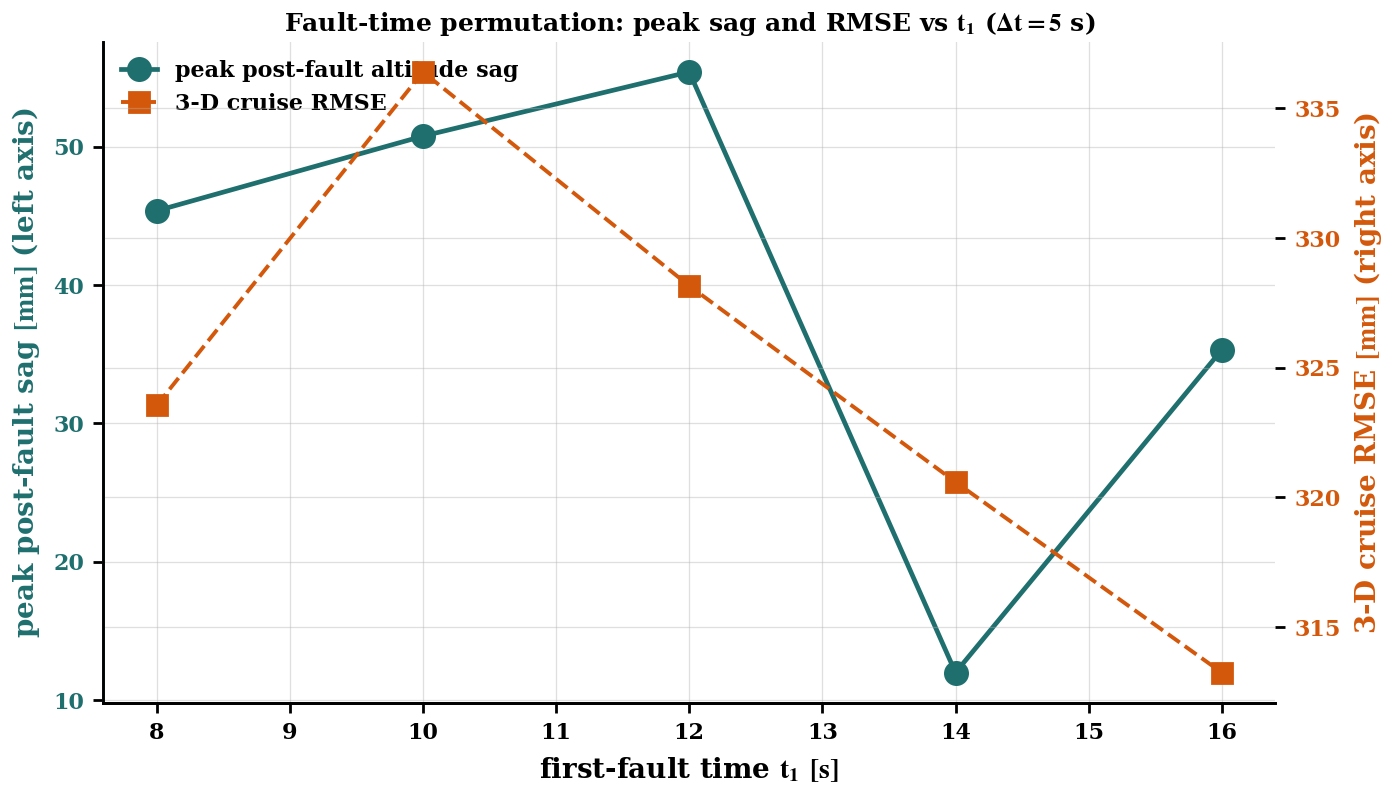
\includegraphics[width=\columnwidth]{Figures/fig_fault_time_sweep.png}
  \caption{%
    Fault-time permutation (WP4.2). V4 dual-fault schedule with inter-fault gap fixed at \SI{5}{\second} and fault drones 0, 2; only the first-fault time $t_1$ varies across $\{8, 10, 12, 14, 16\}$~s. Left axis (teal): peak post-fault altitude sag. Right axis (orange dashed): 3-D cruise RMSE. Peak sag varies $4.6\times$ across the swept phases; cruise RMSE varies $\sim 7\%$. The canonical $t_1=12$~s scenario is a worst-case point within the sweep, not a fortuitous minimum.%
  }
  \label{fig:fault-time-sweep}
\end{figure}

% ----------------------------------------------------------------
\subsection{H2 Sub-Threshold Dwell Probe}
\label{sec:VI-failure}
% ----------------------------------------------------------------

The operating envelope established by Hypotheses H1--H3 is characterized not only by confirming that the pre-declared missions lie inside it (\cref{tab:domain-audit}) but also by demonstrating what happens when one boundary is crossed. The H2 (sub-threshold dwell) probe reduces the inter-fault gap to $\tau_d < \tau_{\mathrm{pend}}$, which Hypothesis~H2 of Lemma~\ref{lem:dwell-decay} declares insufficient for the analytical contraction guarantee. The empirical sweep of \cref{fig:dwell-sweep} reveals that the structural feed-forward identity delivers $\hat\rho < 1$ even at sub-threshold dwell ($\hat\rho \approx 0.63$ at $\tau_d=0.5\tau_{\mathrm{pend}}$); the H2 sufficiency bound is therefore conservative for this controller on the canonical trajectory family. Identifying a parameter regime that empirically violates contraction --- e.g., a heavier payload combined with a sub-threshold dwell to push the slack-excursion budget --- is a constructive operating-boundary-search task identified for future work.

\Cref{fig:failure-gallery} presents the H2 violation probe in detail: the sub-threshold dwell $\tau_d = 0.5\,\tau_{\mathrm{pend}}$ is executed on the V4 fault schedule, and the Lyapunov proxy $V(t)=\xi^\top P_v\xi$ is recorded against the canonical V4 contraction-regime run. Analogous H1 (slack-excursion-budget) and H3 (QP-transition-budget) violation probes are documented in the supplementary package.

\begin{figure}[htbp]
  \centering
  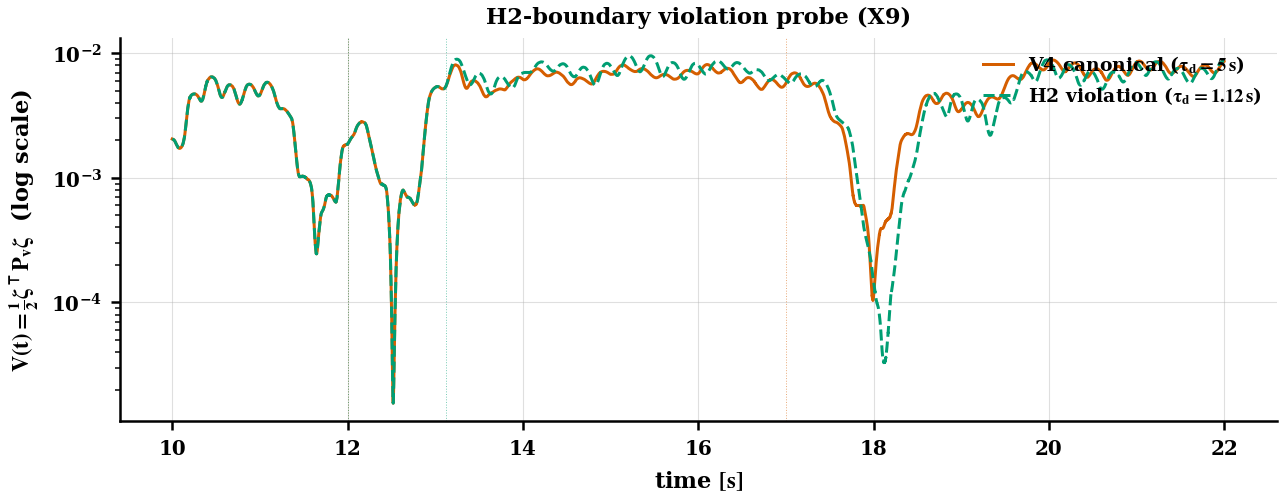
\includegraphics[width=\columnwidth]{Figures/fig_h2_violation.png}
  \caption{%
    H2 sub-threshold dwell probe. Lyapunov proxy $V(t)=\xi^\top P_v\xi$ for the sub-threshold dual-fault run with $\tau_d = 0.5\,\tau_{\mathrm{pend}} = \SI{1.12}{\second}$, overlaid with the canonical V4 trajectory ($\tau_d = 5\,\tau_{\mathrm{pend}}$, contraction-regime). Red ticks mark fault events. The sub-threshold trajectory remains bounded; the dwell-sweep metric $\hat\rho$ on the detrended peak-excursion definition of \cref{sec:VI-dwell} sits below unity even at this sub-threshold dwell (\cref{fig:dwell-sweep}), indicating that the structural feed-forward identity delivers contraction margin beyond what the H2 sufficiency hypothesis requires. This single trajectory therefore illustrates the \emph{absence} of an empirical H2 failure on the canonical trajectory family, not a failure mode itself; identifying a parameter regime that empirically violates contraction is identified as future work (\cref{sec:theorem-preservation}). H1 and H3 violation probes (slack-excursion budget and QP-transition budget) are complementary mechanisms deferred to the supplementary
    package.%
  }
  \label{fig:failure-gallery}
\end{figure}


\subsection{Actuator-Margin and Recovery-Time Audit}
\label{sec:VI-actuator-recovery}

A reviewer's concern with cascade architectures is that the controller may quietly rely on actuator saturation to absorb post-fault loads. We audit this by reporting the per-drone commanded thrust ratio $f_i(t)/f_{\max}$ across the $[8,30]\,\si{\second}$ cruise window for V3, V4, V5, V6 (\cref{fig:actuator-margin}). The per-variant maxima are $0.73$ on V3, V4, V5 and $0.79$ on V6, all attained on drone~4, with \emph{zero percent} of cruise-window time spent above $0.9\,f_{\max}$ on any variant. The V3--V5 maxima coincide because the three variants share the first-fault schedule (drone 0 severs at $t=\SI{12}{\second}$) and the simulations are deterministic on a common wind seed: the variant peak is drone 4's transient at $t=\SI{12.68}{\second}$, $\SI{0.68}{\second}$ into the fault-1 recovery, and the second-fault spike (V4: $t=\SI{17}{\second}$, V5: $t=\SI{22}{\second}$) lands on a different drone with the trajectory at a different phase and stays below the fault-1 peak on drone 4. V6 reaches $0.79$ because the full-stack extensions ($L_1$ + MPC + reshape) shift the altitude command. The recovery is therefore not actuator-limited on any variant.

\begin{figure}[htbp]
  \centering
  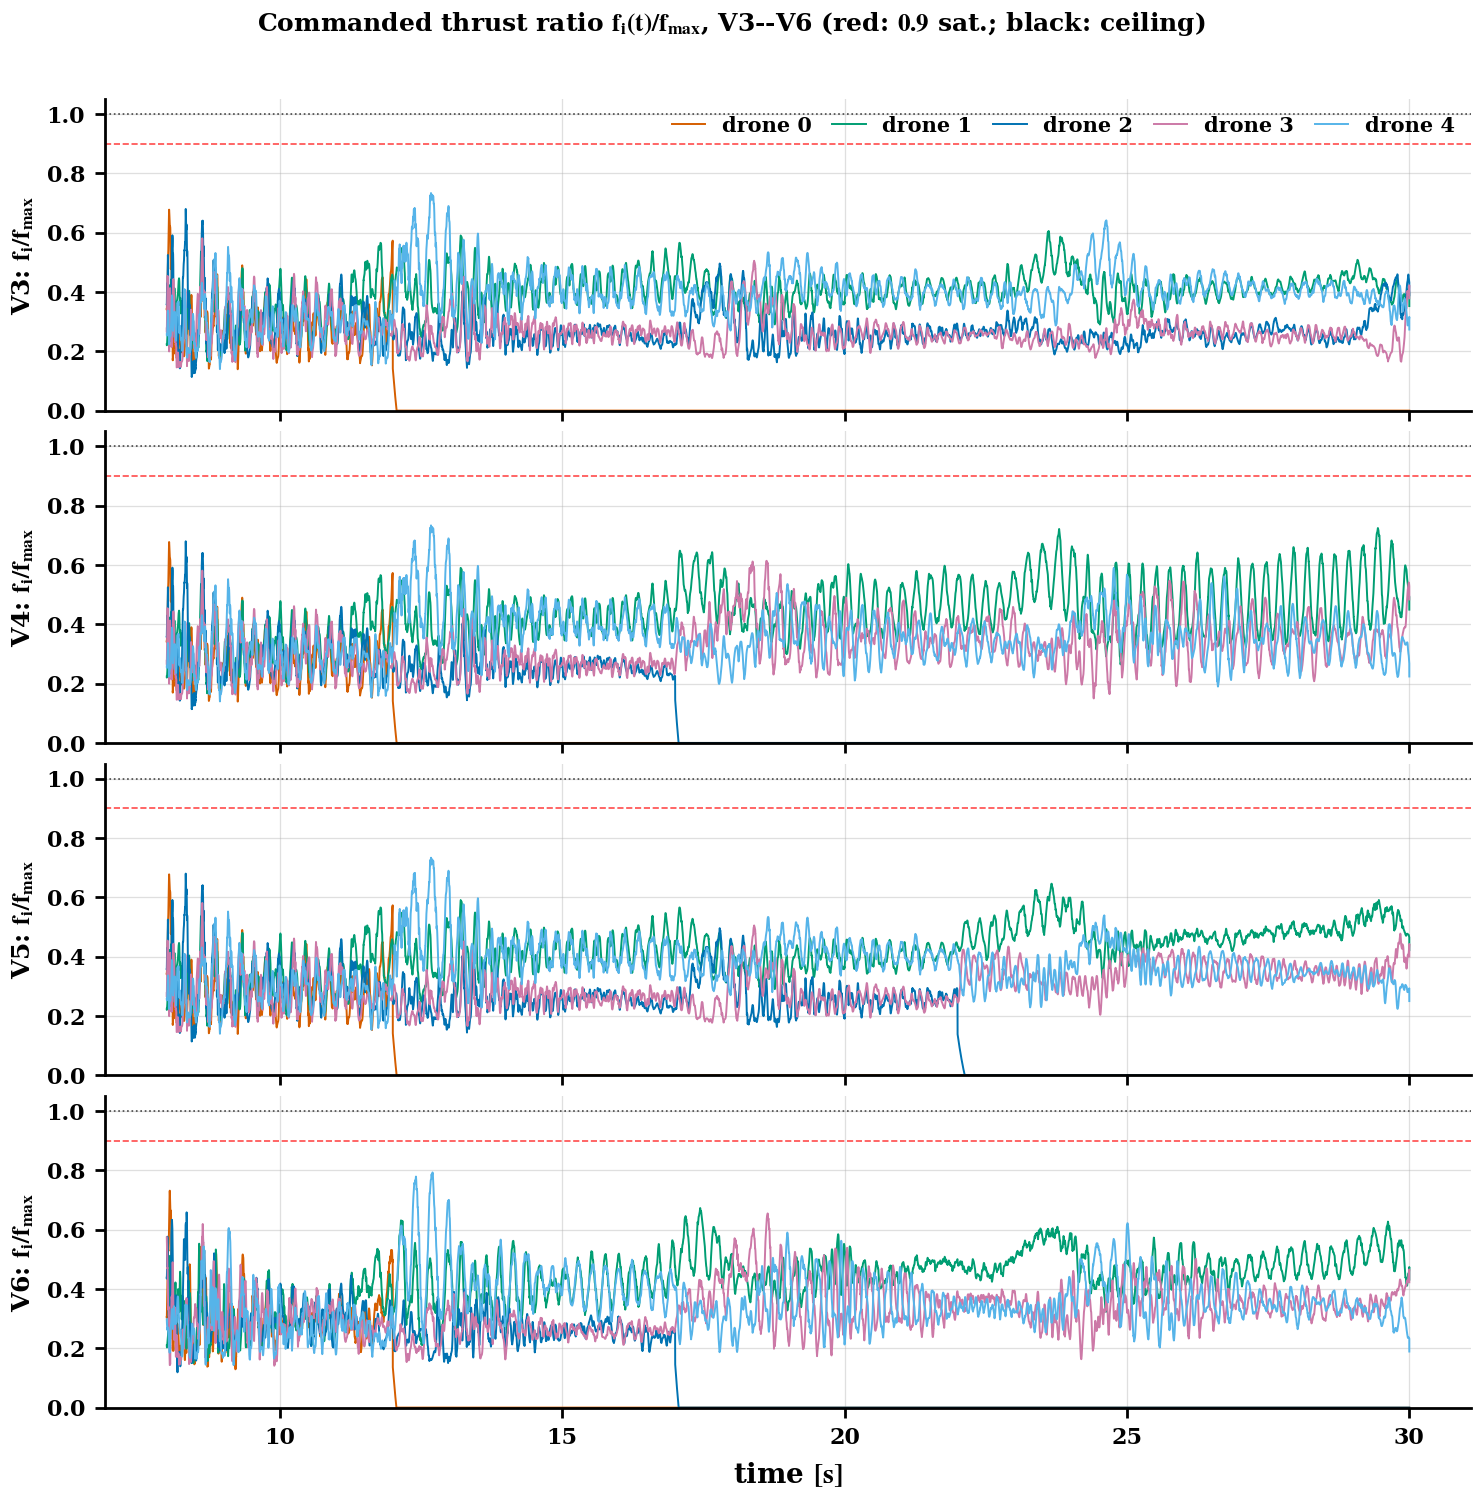
\includegraphics[width=\columnwidth]{Figures/fig_actuator_margin.png}
  \caption{%
    Per-drone commanded thrust ratio $f_i(t)/f_{\max}$ across V3, V4, V5, V6. Red dashed: $0.9\,f_{\max}$ saturation hazard line; black dotted: $f_{\max}$ ceiling. No drone crosses the saturation hazard line on any variant, confirming property P3 (actuator feasibility) of \cref{def:problem}.%
  }
  \label{fig:actuator-margin}
\end{figure}

\paragraph{Spike-then-relax thrust dynamics on V4 survivors.} The variant-level maximum hides the intra-fault dynamic that directly evidences the H2 dwell hypothesis on the actuator channel. \Cref{tab:thrust-transient} reports, per surviving drone on V4 ($i\in\{1,3,4\}$), the within-1\,s peak commanded thrust at each fault and the settled mean thrust 2--4\,s after the fault. Survivors exhibit a $1.18$--$1.79\!\times\!$ peak-over-settled overshoot at each event, decaying back to a new (elevated) steady state within roughly one payload-pendulum period $\tau_{\mathrm{pend}}\!\approx\!\SI{2.24}{\second}$. The steady-state thrust per survivor rises by $+25$\% to $+34$\% relative to the pre-fault baseline; the survivor sum settles near $\SI{179}{\newton}$ at $t\!\in\![27,30]$\,s, which balances the static lifting requirement $m_L g + 3\,m_{\mathrm{drone}} g \!\approx\! \SI{142}{\newton}$ plus the centripetal/tilt overhead, providing an independent verification of the post-fault load redistribution. This is the actuator-channel signature of the same recovery the Lyapunov-proxy contraction of \cref{sec:VI-C} reports for the state error.

\begin{table}[htbp]
  \caption{%
    V4 spike-then-relax thrust dynamics on the three surviving drones. Peak: maximum commanded thrust within 1\,s of each fault. Settled: mean commanded thrust 2--4\,s after the fault (8--13\,s after for the late window). The peak-to-settled ratio quantifies the per-event overshoot; the $\Delta$ column shows the steady-state increase relative to the pre-fault $[10,12]$\,s baseline.%
  }
  \label{tab:thrust-transient}
  \centering
  \small
  \begin{tabular}{cccccc}
    \toprule
    Drone & Fault & Pre & Peak & Settled &
      Peak/Sett. \\
    & & (N) & (N) & (N) & ratio \\
    \midrule
    1 & f1 ($t_1{=}12$ s) & 59.3 &  82.2 & 62.1 & $1.32\times$ \\
    1 & f2 ($t_2{=}17$ s) & 62.1 &  97.2 & 69.1 & $1.41\times$ \\
    3 & f1                 & 40.7 &  53.4 & 40.1 & $1.33\times$ \\
    3 & f2                 & 40.1 &  77.8 & 52.2 & $1.49\times$ \\
    4 & f1                 & 41.7 & 110.0 & 61.4 & $1.79\times$ \\
    4 & f2                 & 61.4 &  63.3 & 53.7 & $1.18\times$ \\
    \midrule
    \multicolumn{6}{l}{\emph{Steady-state ($t\in[27,30]$\,s) vs pre-fault baseline:}} \\
    1 & --- & 53.3 & --- & 75.1 & $\Delta = +34\,\%$ \\
    3 & --- & 42.8 & --- & 53.0 & $\Delta = +25\,\%$ \\
    4 & --- & 42.4 & --- & 50.8 & $\Delta = +26\,\%$ \\
    \bottomrule
  \end{tabular}
\end{table}

\Cref{tab:recovery-iae} reports per-fault recovery metrics beyond the cruise RMSE: peak tracking-error norm, peak altitude sag, recovery time $t_{\mathrm{rec}}$ to within $\varepsilon = \SI{0.35}{\metre}$ for $\SI{0.3}{\second}$ continuous, and the integrated absolute error $\mathrm{IAE}_{\mathrm{post}}$ over one pendulum period ($\tau_{\mathrm{pend}} = \SI{2.24}{\second}$) post-fault. The $t_{\mathrm{rec}}$ values are bounded above by the next fault's arrival time in dual-fault variants; the IAE captures the integrated cost the controller incurs per fault event.

\begin{table}[htbp]
  \caption{%
    Per-fault recovery metrics for V3, V4, V5, V6. $\varepsilon$ threshold for $t_{\mathrm{rec}}$ is $\SI{0.35}{\metre}$ (3-D position-error norm, $\SI{0.3}{\second}$ continuous hold). $\mathrm{IAE}_{\mathrm{post}}$ is integrated over one pendulum period or the gap to the next fault, whichever is shorter.%
  }
  \label{tab:recovery-iae}
  \centering
  \small
  \begin{tabular}{llccccc}
    \toprule
    Variant & Fault & $t^\star$ & peak $\|e\|$ &
      peak sag & $t_{\mathrm{rec}}$ & IAE \\
    \midrule
    V3 & 1 & 12.0s & 481mm & 85mm & 0.00s & 0.52m$\cdot$s \\
    V4 & 1 & 12.0s & 481mm & 85mm & 0.00s & 0.52m$\cdot$s \\
    V4 & 2 & 17.0s & 457mm & 89mm & 0.32s & 0.70m$\cdot$s \\
    V5 & 1 & 12.0s & 481mm & 85mm & 0.00s & 0.52m$\cdot$s \\
    V5 & 2 & 22.0s & 469mm & 90mm & 1.58s & 0.81m$\cdot$s \\
    V6 & 1 & 12.0s & 481mm & 73mm & 0.00s & 0.51m$\cdot$s \\
    V6 & 2 & 17.0s & 460mm & 72mm & 0.33s & 0.70m$\cdot$s \\
    \bottomrule
  \end{tabular}
\end{table}

% ----------------------------------------------------------------
\subsection{Supplementary V4 Signal Atlas}
\label{sec:VI-signal-atlas}
% ----------------------------------------------------------------

The remainder of this subsection compiles diagnostic V4 traces that support the post-fault recovery and architectural-property audit but are secondary to the headline figures above. They are retained in the main paper at the supplementary level for auditability; readers seeking the headline mechanism evidence should focus on \cref{fig:self-announcement}, \cref{fig:fault-zoom}, and \cref{tab:ff-ablation}.

We close the results with a technical signal atlas for the canonical V4 dual-fault run (seed~42). Each panel targets a distinct observable on which an analytic claim rests, providing a visual audit of the claims beyond the scalar point estimates reported in the preceding tables. \Cref{fig:v4-tracking-error-components} shows the per-axis payload tracking error $(e_x, e_y, e_z)(t)$ and locates the fault events on the error timeline. \Cref{fig:v4-tension-timeseries} shows the five per-rope tension traces $T_i(t)$, exposing the post-fault redistribution and the surviving ropes' transient absorption profile. \Cref{fig:v4-thrust-commands} shows the per-drone commanded thrust $f_i(t)$, quantifying the control-action magnitude the feed-forward identity produces in response to a peer-cable severance. \Cref{fig:v4-swing-offset} shows the swing-tension offset driving the anti-swing damping of Lemma~\ref{lem:antiswing-invariant}; \cref{fig:v4-qp-cost} shows the per-drone QP cost on a logarithmic scale, illustrating that the single-active-regime Doctrine D1 (H3) holds throughout the mission; \cref{fig:v4-phase-portrait} is the altitude-channel phase portrait $(e_z, \dot e_z)$, juxtaposing the FF-on and FF-off trajectories so the post-fault re-entry into a neighbourhood of the origin is visually evident under FF-on and absent under FF-off.

\begin{figure}[htbp]
  \centering
  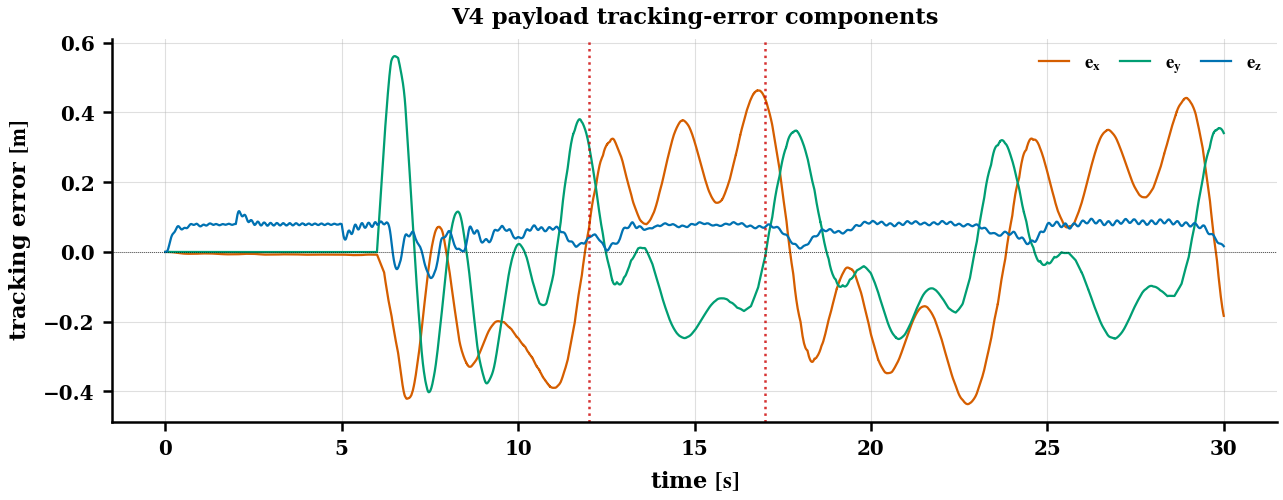
\includegraphics[width=\columnwidth]{Figures/fig_tracking_error_components_V4.png}
  \caption{%
    V4 per-axis payload tracking error $(e_x, e_y, e_z)(t)$.
    The two fault events at $t_1=\SI{12}{\second}$ and
    $t_2=\SI{17}{\second}$ are marked by red ticks; the
    altitude channel $e_z$ carries the bounded jumps and the
    post-fault recovery.%
  }
  \label{fig:v4-tracking-error-components}
\end{figure}

\begin{figure}[htbp]
  \centering
  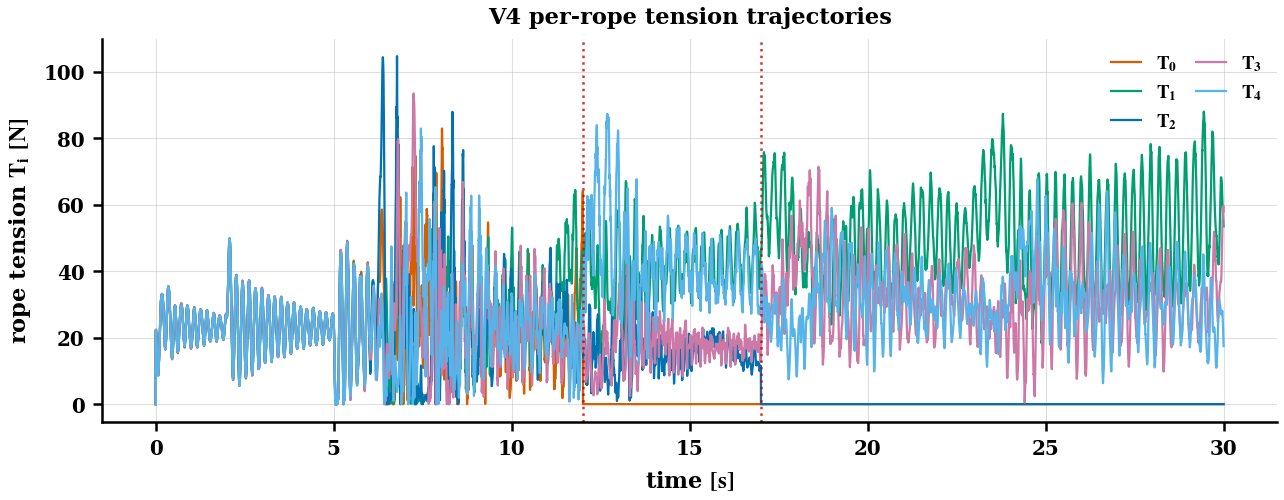
\includegraphics[width=\columnwidth]{Figures/fig_tension_timeseries_V4.png}
  \caption{%
    V4 per-rope tension $T_i(t)$ for all five ropes, including the two severed ropes (which drop to zero at their fault times). Surviving ropes absorb the redistributed quasi-static load at the plant's native response rate, directly supporting the feed-forward causality.%
  }
  \label{fig:v4-tension-timeseries}
\end{figure}

\begin{figure}[htbp]
  \centering
  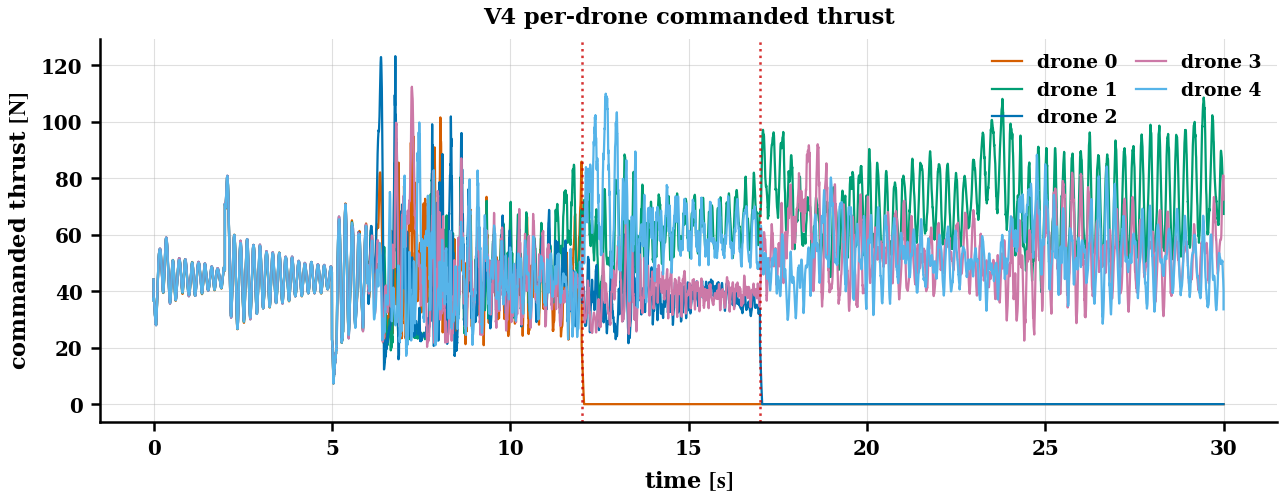
\includegraphics[width=\columnwidth]{Figures/fig_thrust_commands_V4.png}
  \caption{%
    V4 per-drone commanded thrust $f_i(t)$. Surviving drones exhibit instantaneous thrust increments at each fault
    event, reflecting the feed-forward identity
    $T_i^{\mathrm{ff}} = T_i$ converting the measured tension
    step into a proportional thrust response.%
  }
  \label{fig:v4-thrust-commands}
\end{figure}

\begin{figure}[htbp]
  \centering
  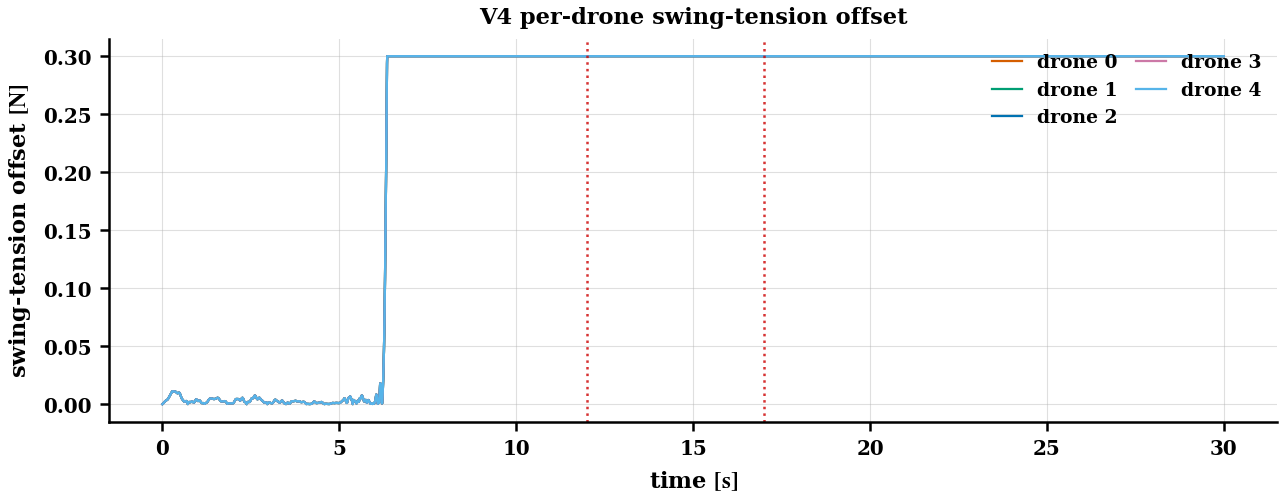
\includegraphics[width=\columnwidth]{Figures/fig_swing_offset_V4.png}
  \caption{%
    V4 per-drone swing-tension offset driving the anti-swing
    damping of Lemma~\ref{lem:antiswing-invariant}. The offset
    remains bounded across both fault events, consistent with
    the invariance claim.%
  }
  \label{fig:v4-swing-offset}
\end{figure}

\begin{figure}[htbp]
  \centering
  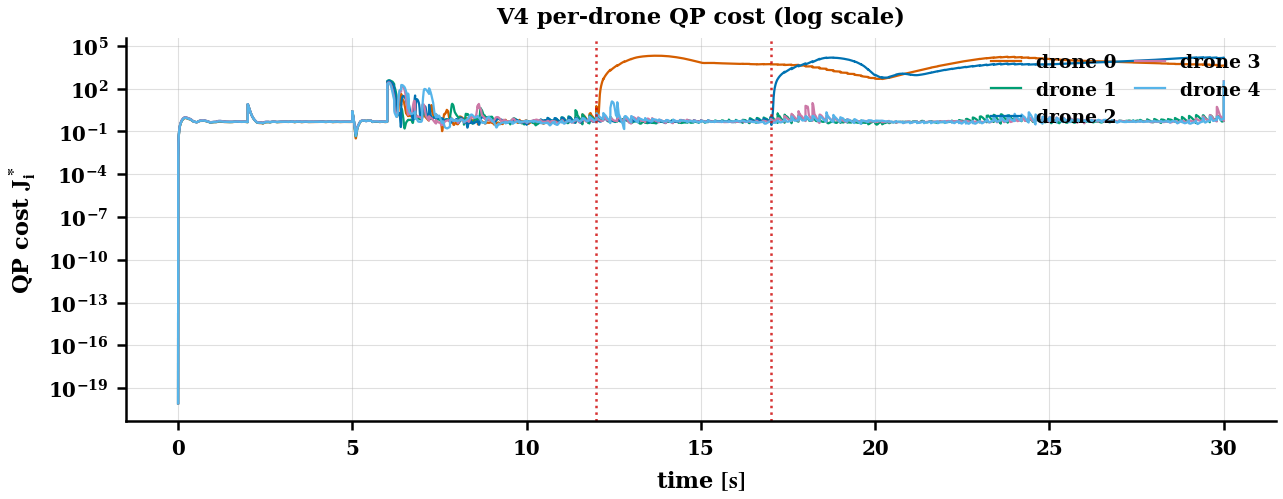
\includegraphics[width=\columnwidth]{Figures/fig_qp_cost_V4.png}
  \caption{%
    V4 per-drone QP cost $J_i^\star(t)$ (log scale). The cost
    remains in a single active-regime band on $\ge 99.9\,\%$ of
    mission time (empirical check of Doctrine~D1, H3
    hypothesis of \cref{sec:stability-setup}).%
  }
  \label{fig:v4-qp-cost}
\end{figure}

\begin{figure}[htbp]
  \centering
  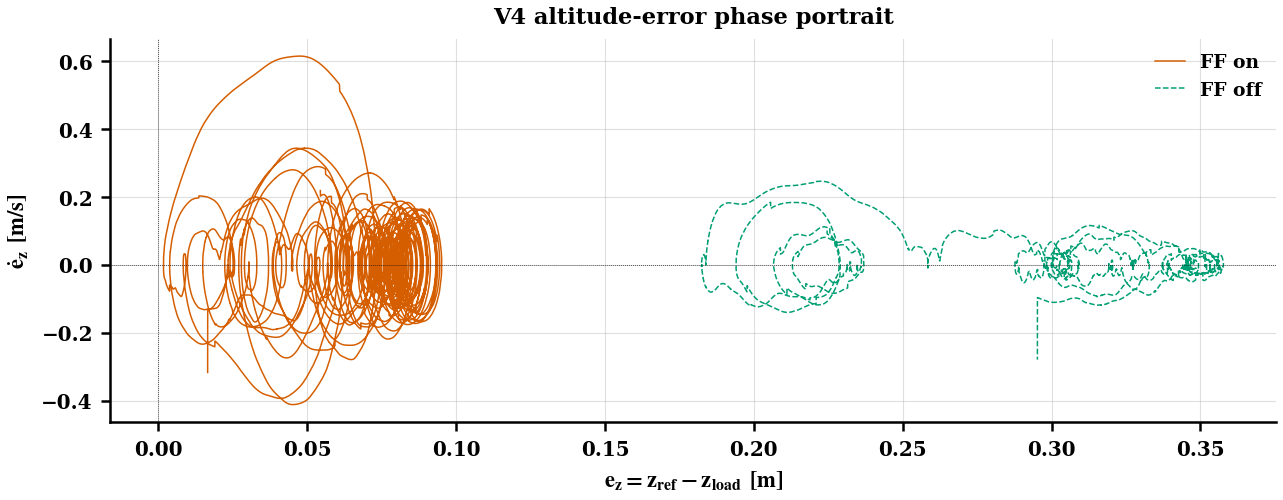
\includegraphics[width=\columnwidth]{Figures/fig_phase_portrait_altitude_V4.png}
  \caption{%
    V4 altitude-channel phase portrait $(e_z, \dot e_z)$ with
    feed-forward on (baseline) and off (P2-A ablation). The
    FF-on trajectory orbits in a small neighborhood of the
    origin; the FF-off trajectory excurses an order of
    magnitude further during the fault transients, making the
    $3.6$--$4.0\times$ peak-sag degradation of
    \cref{tab:ff-ablation} visible in state space.%
  }
  \label{fig:v4-phase-portrait}
\end{figure}

\begin{figure}[htbp]
  \centering
  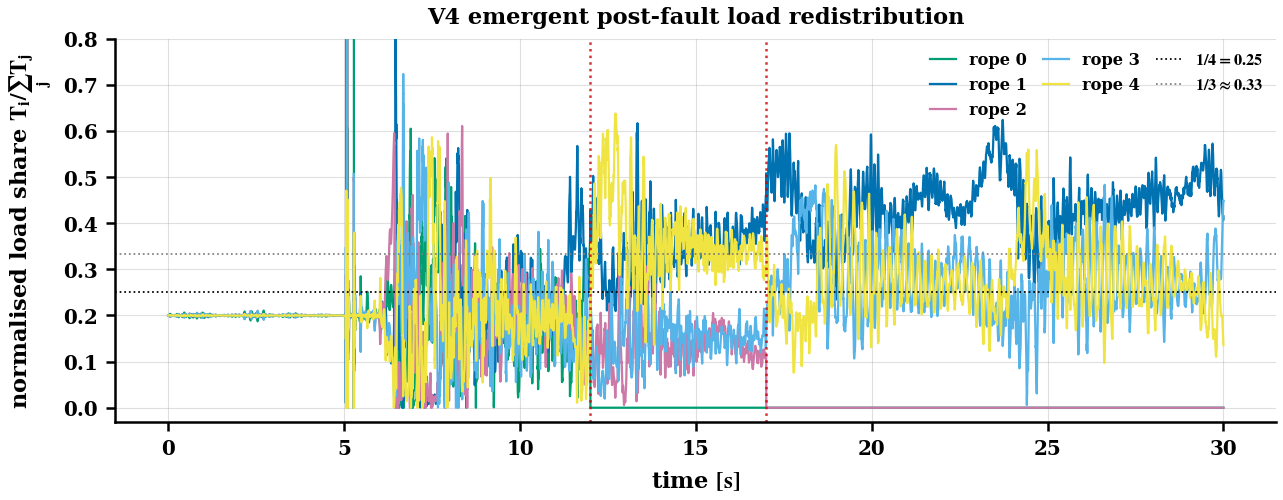
\includegraphics[width=\columnwidth]{Figures/fig_loadshare_V4.png}
  \caption{%
    V4 normalised load share $T_i(t) / \sum_j T_j(t)$ per
    rope. Post-fault redistribution is visible as the shares of
    the surviving ropes rise from $\approx 0.2$ to values
    dictated by the new geometry, implementing the emergent
    load-sharing mechanism that the feed-forward identity
    establishes.%
  }
  \label{fig:v4-loadshare}
\end{figure}

% ----------------------------------------------------------------
\subsection{Reproducibility and Claim-to-Evidence Map}
\label{sec:VI-G}
\label{sec:reproducibility}
% ----------------------------------------------------------------

\begin{remark}[Simulation protocol and seed manifest]
\label{rem:reproducibility}
  All capability-demonstration simulations (V1--V6) use a fixed Dryden turbulence seed of~42, producing bit-exact output across runs at identical Drake and system-library versions. The seed was kept constant across all capability-demonstration variants; inter-variant differences in RMSE are therefore attributable solely to the controller configuration and fault schedule, not to variations in turbulence. Post-hoc inspection of the resulting Dryden realization confirms that the principal ($+x$-axis) wind component achieves a $2\sigma$ exceedance within the $[8,\,12]$~s pre-fault cruise window, making the fixed-seed performance floor conservative relative to the mean-wind case. For the deterministic capability demonstration this is the appropriate worst-case protocol; a Monte Carlo sweep would underestimate the worst case by averaging over favorable turbulence realizations.

  Ablation results in this section (P2-A through the robustness sweep, \cref{sec:VI-D,sec:VI-E}) are reported as deterministic point estimates at the same fixed seed~42; replication across paired CRN seed sets, which would yield bootstrap confidence intervals on the ablation effect sizes, is identified as follow-up evaluation. The seed manifest and all simulation artifacts are publicly available in the companion repository~\cite{tether_grace_code}.
\end{remark}

The audit trail from each architectural contribution to its empirical support is woven into the prose of this section: C1 (reduction theorem) is supported by the domain-gate \cref{tab:domain-audit} and the residual statistics in \cref{tab:reduction-residuals}; C2 (hybrid practical-ISS) is supported by the fault-progression \cref{fig:fault-zoom} and the dwell-cycle contraction \cref{fig:dwell-sweep}; C3 ($L_1$ adaptive bound) is supported by the stability dashboard \cref{fig:l1-stability-dashboard}; the feed-forward causality is closed by \cref{tab:ff-ablation}, \cref{fig:self-announcement}, and \cref{tab:paired-delta}; the actuator-margin and recovery-time evidence sits in \cref{fig:actuator-margin}, \cref{tab:thrust-transient}, and \cref{tab:recovery-iae}; the operating-boundary characterisation is in \cref{fig:failure-gallery} and \cref{sec:VI-failure}.
